
\documentclass[12pt,a4paper]{article}

%-----------------------------------------------
% PAGE LAYOUT
%-----------------------------------------------
\usepackage[a4paper,
            left=1in,
            right=1in,
            top=1in,
            bottom=1in]{geometry}

\usepackage{ragged2e}
\usepackage{xurl}
\usepackage[hidelinks]{hyperref}
\urlstyle{same}
%-----------------------------------------------
% FONT AND TEXT FORMATTING
%-----------------------------------------------
\usepackage[T1]{fontenc}
\usepackage{newtxtext,newtxmath}
\usepackage{microtype}
\usepackage{setspace}
\usepackage{svg}

\onehalfspacing
\setlength{\parindent}{0.3in}
\setlength{\parskip}{5pt}

%-----------------------------------------------
% MATHEMATICAL PACKAGES
%-----------------------------------------------
\usepackage{amsmath}
\usepackage{amssymb}
\usepackage{mathtools}

%-----------------------------------------------
% IMAGES AND FIGURES
%-----------------------------------------------
\usepackage{graphicx}
\usepackage{float}
\usepackage{caption}
\usepackage{subcaption}
\usepackage{graphicx}
\usepackage{caption}
\usepackage{float}

\graphicspath{{graph_images/}}

\captionsetup{
    font=small,
    labelfont=bf,
    justification=centering
}

%-----------------------------------------------
% TABLE FORMATTING
%-----------------------------------------------
\usepackage{booktabs}
\usepackage{tabularx}
\usepackage{array}
\usepackage{longtable}

%-----------------------------------------------
% LIST FORMATTING
%-----------------------------------------------
\usepackage{enumitem}

\setlist[itemize]{
    leftmargin=0.35in,
    itemsep=3pt
}

\setlist[enumerate]{
    leftmargin=0.4in,
    itemsep=4pt
}

%-----------------------------------------------
% SECTION HEADING FORMATTING
%-----------------------------------------------
\usepackage{titlesec}
\usepackage{xcolor}

\definecolor{headingblue}{RGB}{25,55,95}
\definecolor{linkblue}{RGB}{30,75,130}

\titleformat{\section}
  {\normalfont\Large\bfseries\color{headingblue}}
  {\thesection.}{0.6em}{}

\titleformat{\subsection}
  {\normalfont\large\bfseries\color{headingblue}}
  {\thesubsection}{0.6em}{}

\titlespacing*{\section}
  {0pt}{18pt}{10pt}

\titlespacing*{\subsection}
  {0pt}{12pt}{6pt}

%-----------------------------------------------
% HEADER AND FOOTER
%-----------------------------------------------
\usepackage{fancyhdr}

\pagestyle{fancy}
\fancyhf{}

\fancyfoot[C]{\thepage}

\pagestyle{plain}

%-----------------------------------------------
% TABLE OF CONTENTS
%-----------------------------------------------
\usepackage{tocloft}

\renewcommand{\contentsname}{TABLE OF CONTENTS}

%-----------------------------------------------
% HYPERLINKS (LOAD NEAR THE END)
%-----------------------------------------------
\usepackage[
    colorlinks=true,
    linkcolor=linkblue,
    urlcolor=linkblue,
    citecolor=linkblue
]{hyperref}


\allowdisplaybreaks

\title{\textbf{Visual Exploration and Structural Analysis of Different Types of Graphs} }


\begin{document}
\justifying

\begin{titlepage}
\begin{center}

\vspace*{0.5cm}

{\Large\textbf{DAYANANDA SAGAR UNIVERSITY}}\\[0.2cm]

{\normalsize School of Engineering}\\
{\normalsize Department of Computer Science and Medical Engineering}\\[1.2cm]

{\Large\textbf{Continuous  Assessment Test 2 }}\\[0.5cm]

\rule{\textwidth}{1 pt}\\[0.4cm]

{\LARGE\bfseries VISUALIZATION AND ANALYSIS OF}\\[0.2cm]
{\LARGE\bfseries DIFFERENT TYPES OF GRAPHS}\\[0.4cm]

\rule{\textwidth}{1 pt}\\[1cm]

{\large\textbf{Subject:}}\\[0.2cm]
{\large Discrete Mathematics \& Graph Theory}\\[0.2cm]
{\large Course Code: 25SM2303}\\[1cm]

\textbf{Submitted by}\\[0.3cm]

\textbf{Student Name:} Kavana S\\
\textbf{USN:}  ENG25SM0002\\
\textbf{Semester/Section:}  3A\\
\textbf{Department:} Computer Science and  Medical Engineering\\[1cm]

\textbf{Submitted to}\\[0.3cm]

Dr. Agughasi Victor Ikechukwu\\
Department of Computer Science and Engineering\\[1cm]

\vfill

{\large Academic Year 2026--2027}

\end{center}
\end{titlepage}

%================================================
% SECTION 1: INTRODUCTION TO GRAPH THEORY
%================================================

\pagenumbering{roman}

\tableofcontents
\newpage

\pagenumbering{arabic}
\setcounter{page}{1}

\section{Introduction to Graph Theory}

Graph theory is an important branch of discrete mathematics
that deals with the study of relationships and connections
between objects. It represents different systems using
vertices and edges, making it easier to understand how
individual elements are connected. Graphs are widely used
in computer networks, social media, transportation systems,
communication networks and many other applications.

A graph is mathematically represented as $G = (V,E)$,
where $V$ represents a non-empty set of vertices and
$E$ represents a set of edges connecting pairs of vertices.
Vertices are also called nodes, while edges represent the
relationships or connections between them. The number of
vertices is called the order of the graph, represented by
$|V|$, and the number of edges is called the size of the
graph, represented by $|E|$.

For example, consider a graph with four vertices
$V = \{A,B,C,D\}$ and four edges
$E = \{AB,BC,CD,DA\}$. These vertices and edges form
a closed structure in which every vertex is connected
to two other vertices. This example helps illustrate how
vertices and edges work together to represent relationships
within a graph.

The basic components of a graph include vertices, edges,
adjacent vertices and incident edges. A vertex represents
an individual object in a system, whereas an edge represents
a connection between two vertices. Two vertices are called
adjacent if an edge directly connects them. An edge is said
to be incident on the vertices that it connects. The degree
of a vertex is the number of edges connected to it. A vertex
with degree zero is called an isolated vertex, while a vertex
with degree one is called a pendant vertex or leaf. These
concepts help describe the structure and connectivity of
a graph.

Another important concept in graph theory is the study of
paths and cycles. A path is a sequence of vertices in which
consecutive vertices are connected by edges. A cycle is a
closed path that starts and ends at the same vertex without
repeating other vertices. Paths and cycles are useful for
analysing routes, communication links and network connections.
They help determine whether one vertex can be reached from
another through a sequence of edges.

Graph theory provides a mathematical method for representing
and analysing complex relationships. In computer networks,
vertices represent computers or routers and edges represent
communication links. In social networks, vertices represent
users and edges represent friendships or interactions.
Similarly, transportation systems use graphs to represent
locations and routes. Therefore, graph theory plays an
important role in solving practical problems involving
connections, paths and network structures.


\section{Types of Graphs}

Graphs are classified into different types based on the
nature of their vertices and edges. Each type represents
a different form of relationship between objects.
Understanding these classifications helps in selecting
the appropriate graph model for a particular problem.

% 2.1 Simple Graph
\subsection{Simple Graph}

\noindent
\begin{minipage}[c]{0.58\textwidth}
A simple graph is an undirected graph that contains no
self-loops and no multiple edges between the same pair
of vertices. Each edge connects two distinct vertices
exactly once. Simple graphs are commonly used to
represent basic relationships, such as friendship
connections in social networks.
\end{minipage}
\hfill
\begin{minipage}[c]{0.36\textwidth}
\centering
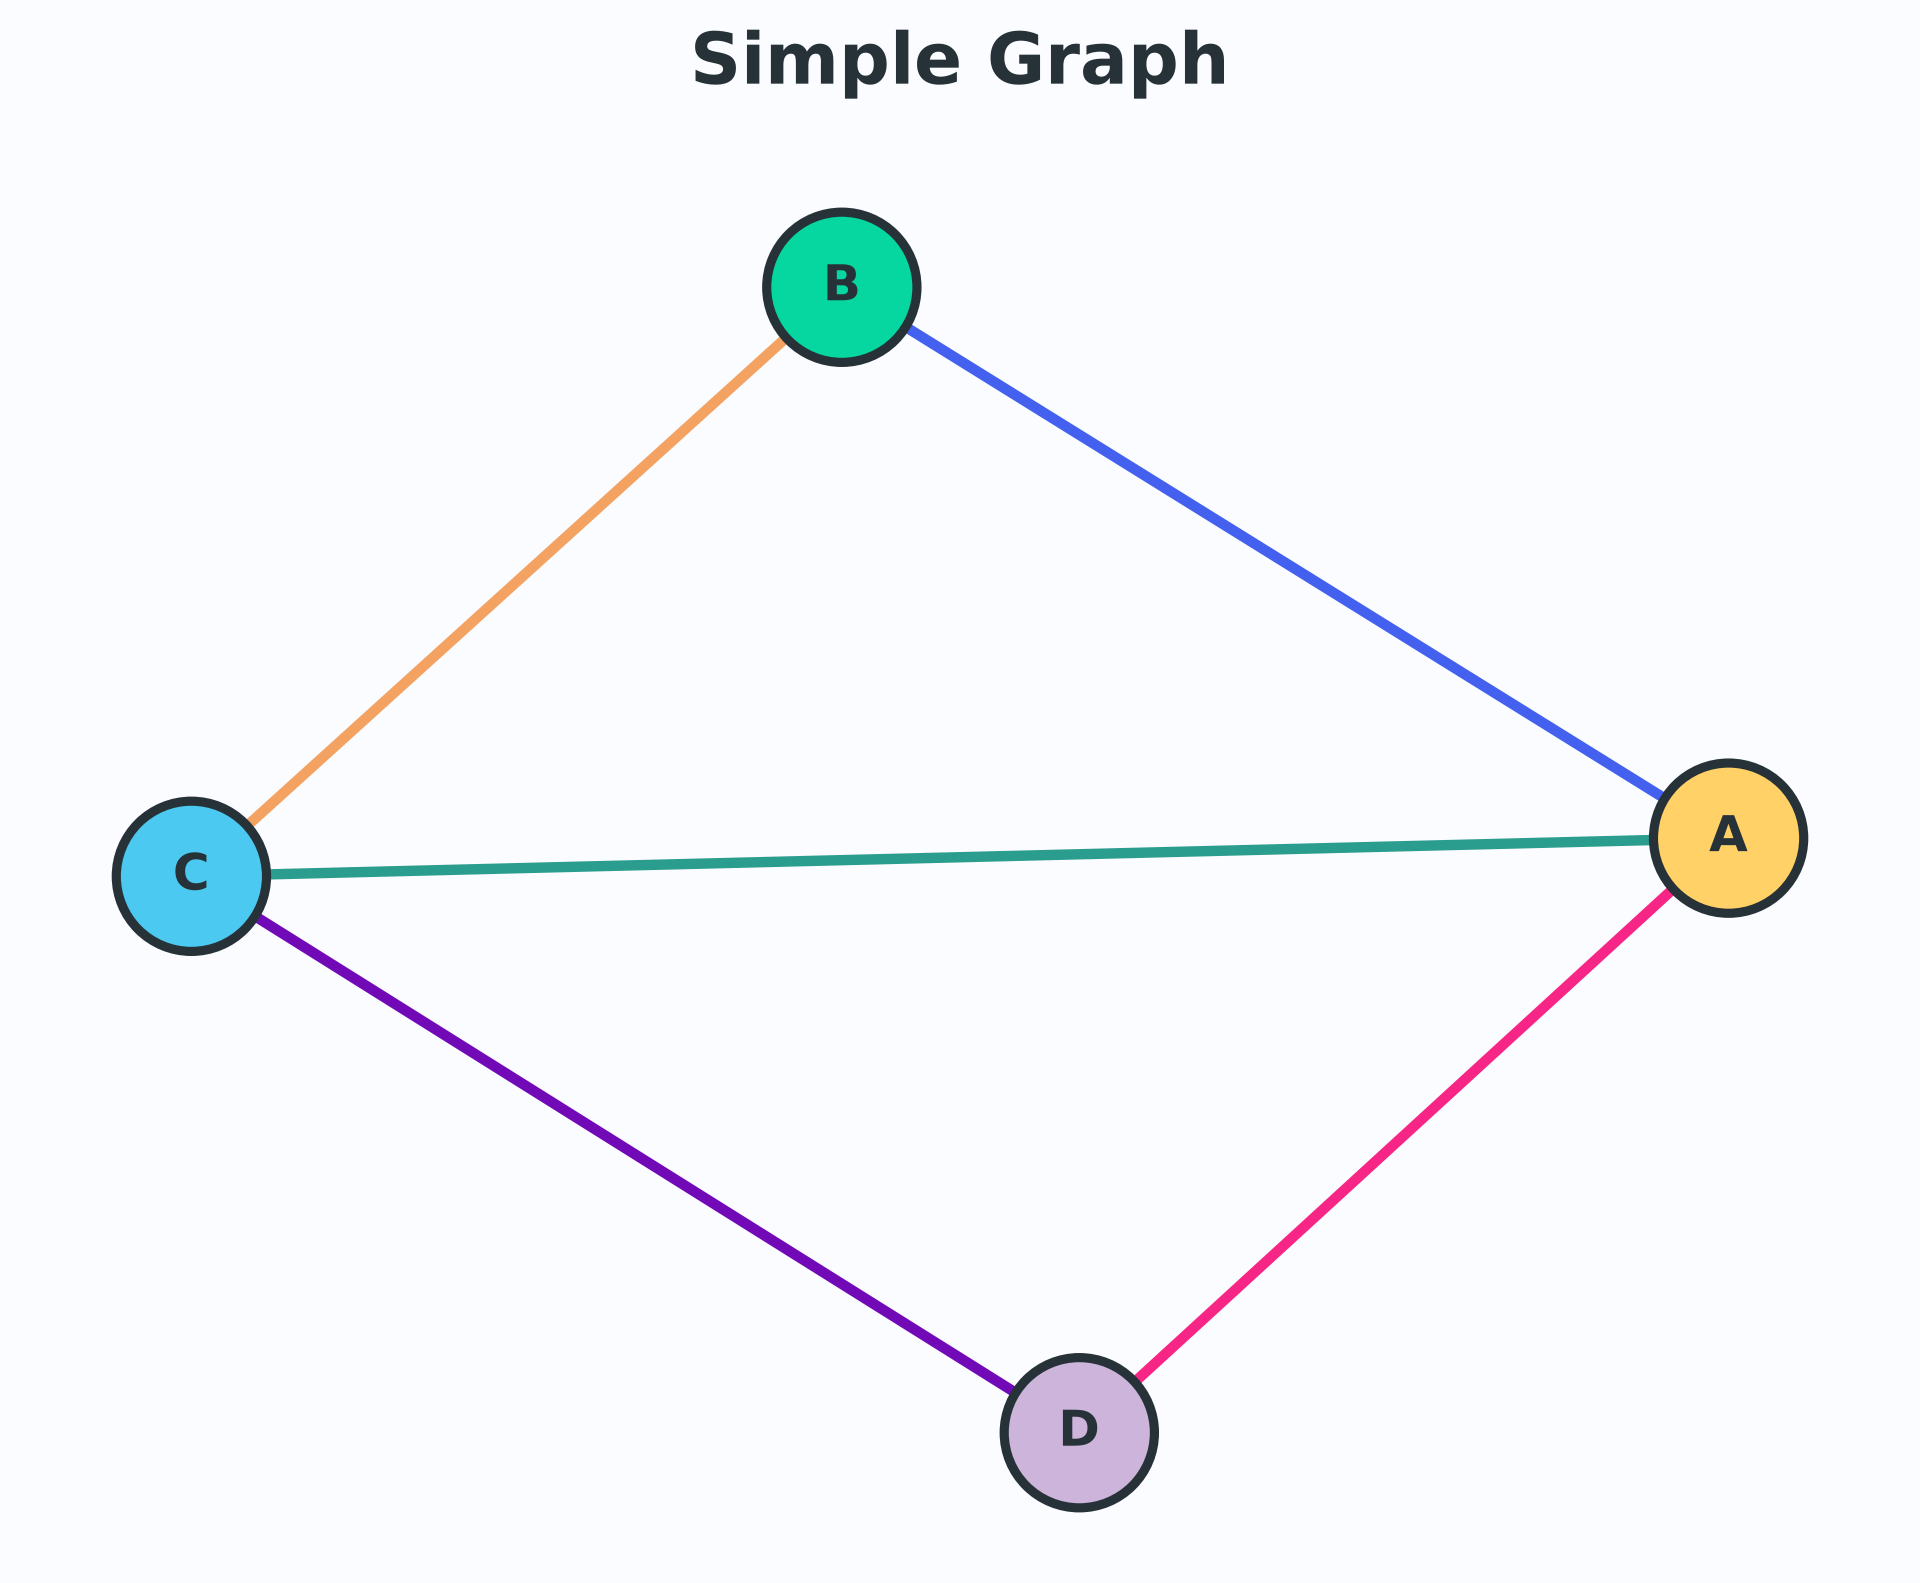
\includegraphics[width=\linewidth,height=4cm,keepaspectratio]
{graph_images/simple_graph.png}
\end{minipage}

\vspace{0.35cm}

% 2.2 Multigraph
\subsection{Multigraph}

\noindent
\begin{minipage}[c]{0.58\textwidth}
A multigraph is a graph in which multiple edges are
allowed between the same pair of vertices. These edges
represent different connections between two objects.
For example, in a transportation network, two cities
may be connected by multiple roads or railway routes.
\end{minipage}
\hfill
\begin{minipage}[c]{0.36\textwidth}
\centering
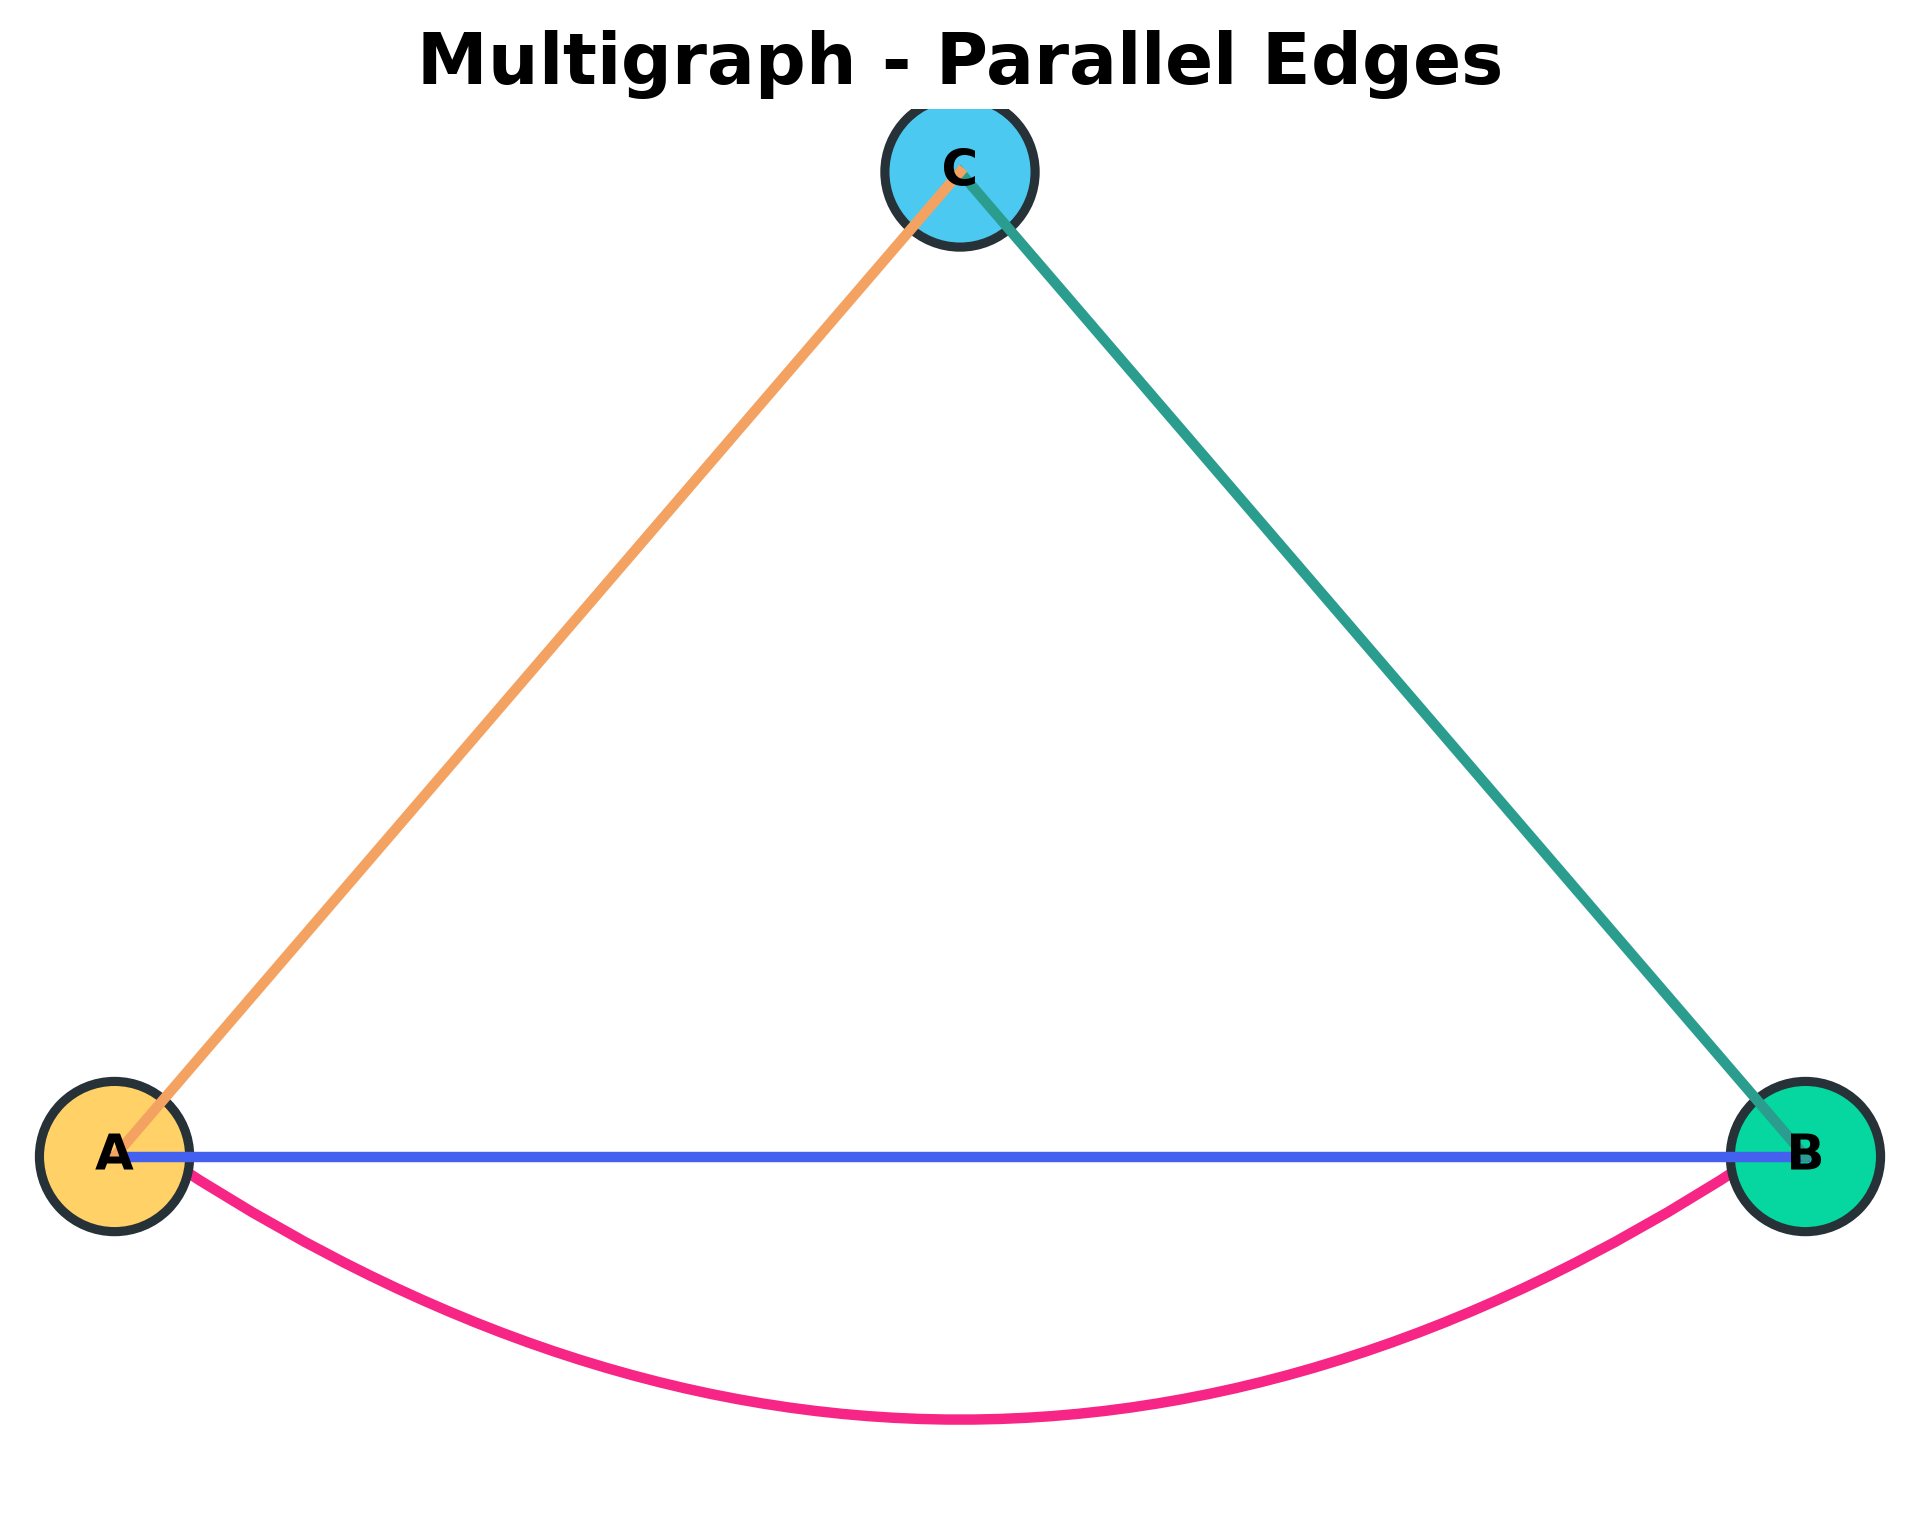
\includegraphics[width=\linewidth,height=4cm,keepaspectratio]
{graph_images/multigraph.png}
\end{minipage}

\vspace{0.35cm}

% 2.3 Pseudograph
\subsection{Pseudograph}

\noindent
\begin{minipage}[c]{0.58\textwidth}
A pseudograph is a graph that allows both multiple
edges and self-loops. A self-loop is an edge that
connects a vertex to itself. Pseudographs are useful
for representing systems in which an object can have
a relationship with itself, along with multiple
connections to other objects.
\end{minipage}
\hfill
\begin{minipage}[c]{0.36\textwidth}
\centering
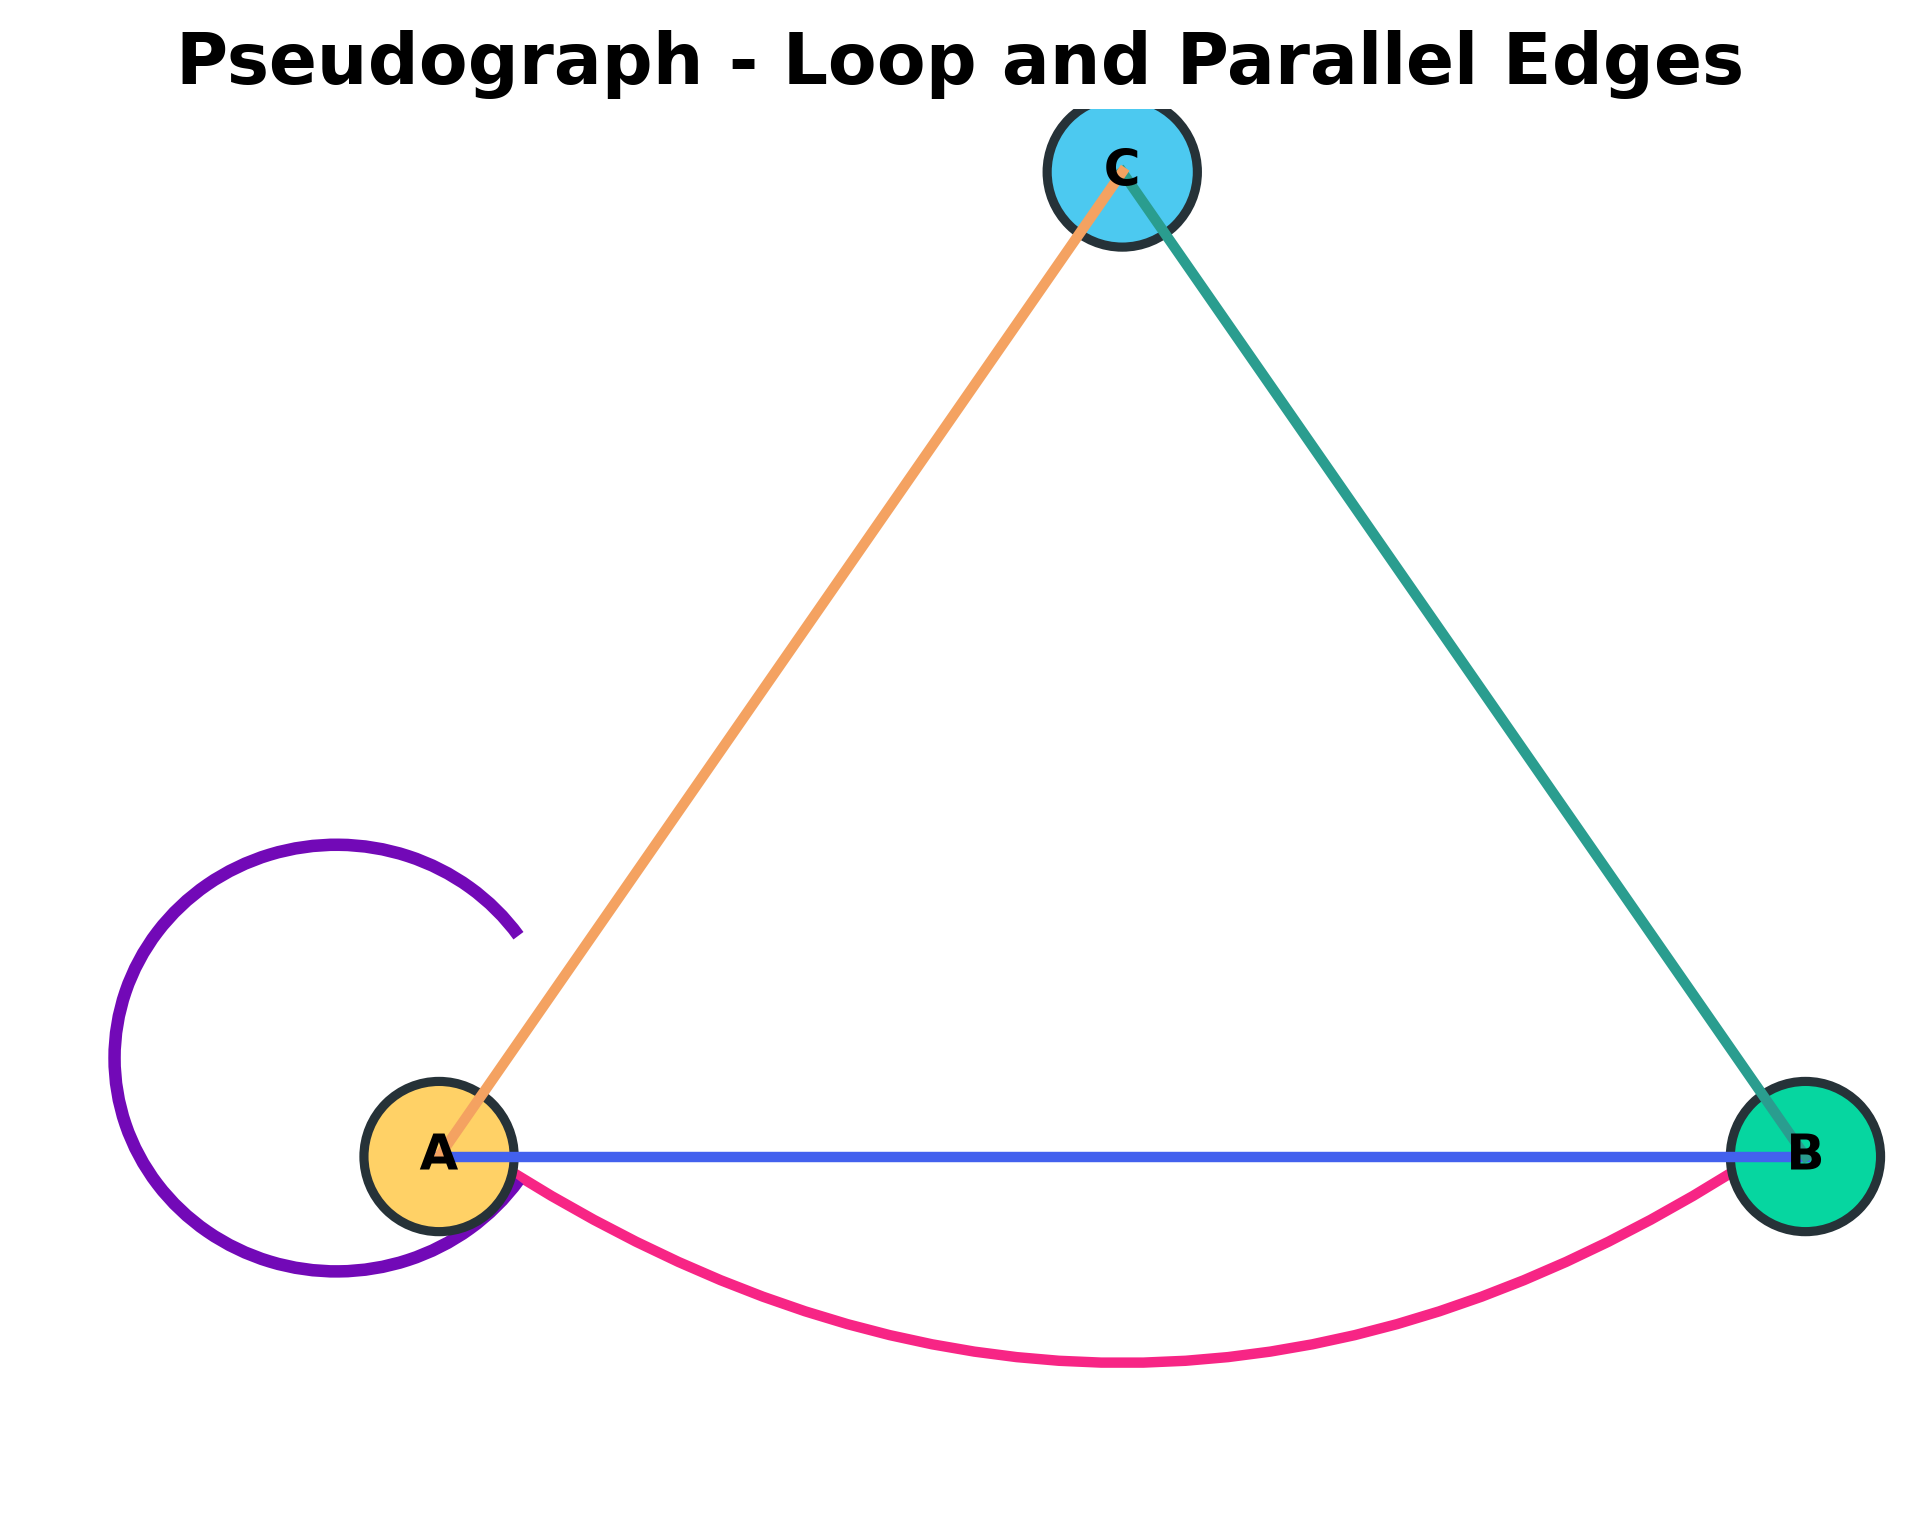
\includegraphics[width=\linewidth,height=4cm,keepaspectratio]
{graph_images/pseudograph.png}
\end{minipage}

\vspace{0.35cm}

% 2.4 Directed Graph
\subsection{Directed Graph}

\noindent
\begin{minipage}[c]{0.58\textwidth}
A directed graph, also called a digraph, is a graph
in which every edge has a specific direction. Directed
edges are represented using arrows, indicating the
direction of the relationship between two vertices.
For example, webpage links and one-way roads can be
represented using directed graphs.
\end{minipage}
\hfill
\begin{minipage}[c]{0.36\textwidth}
\centering
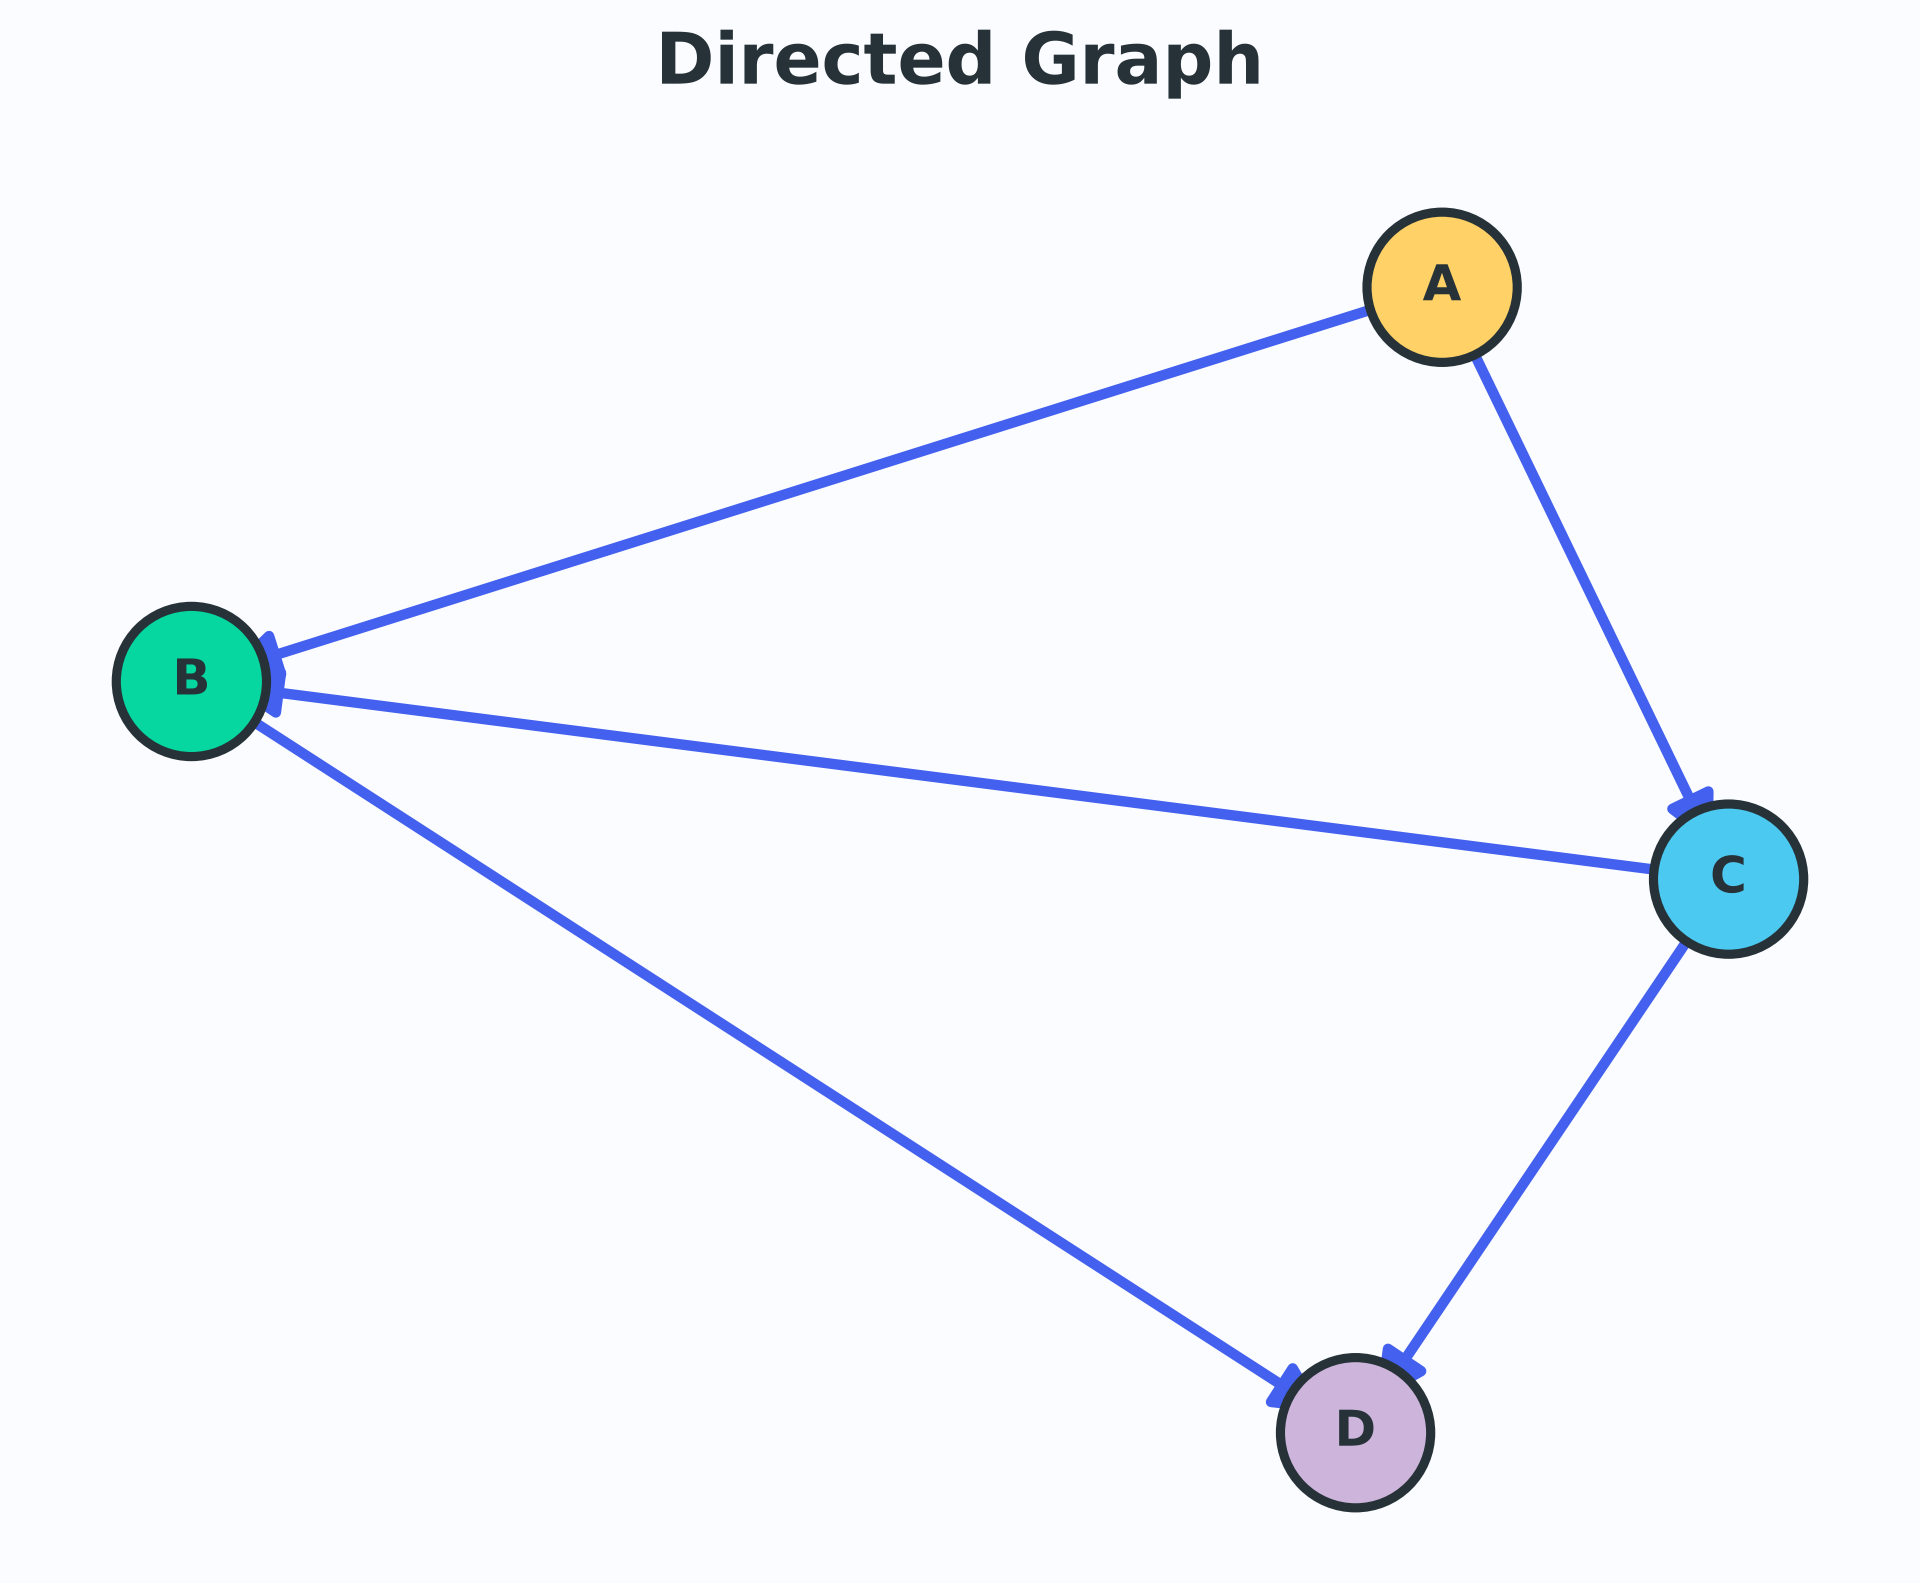
\includegraphics[width=\linewidth,height=4cm,keepaspectratio]
{graph_images/directed_graph.png}
\end{minipage}

\vspace{0.35cm}

% 2.5 Undirected Graph
\subsection{Undirected Graph}

\noindent
\begin{minipage}[c]{0.58\textwidth}
An undirected graph is a graph in which edges do not
have any specific direction. The connection between
two vertices works in both directions. For example,
a mutual friendship between two people can be
represented using an undirected edge. These graphs
are commonly used in social networks and two-way
communication systems.
\end{minipage}
\hfill
\begin{minipage}[c]{0.36\textwidth}
\centering
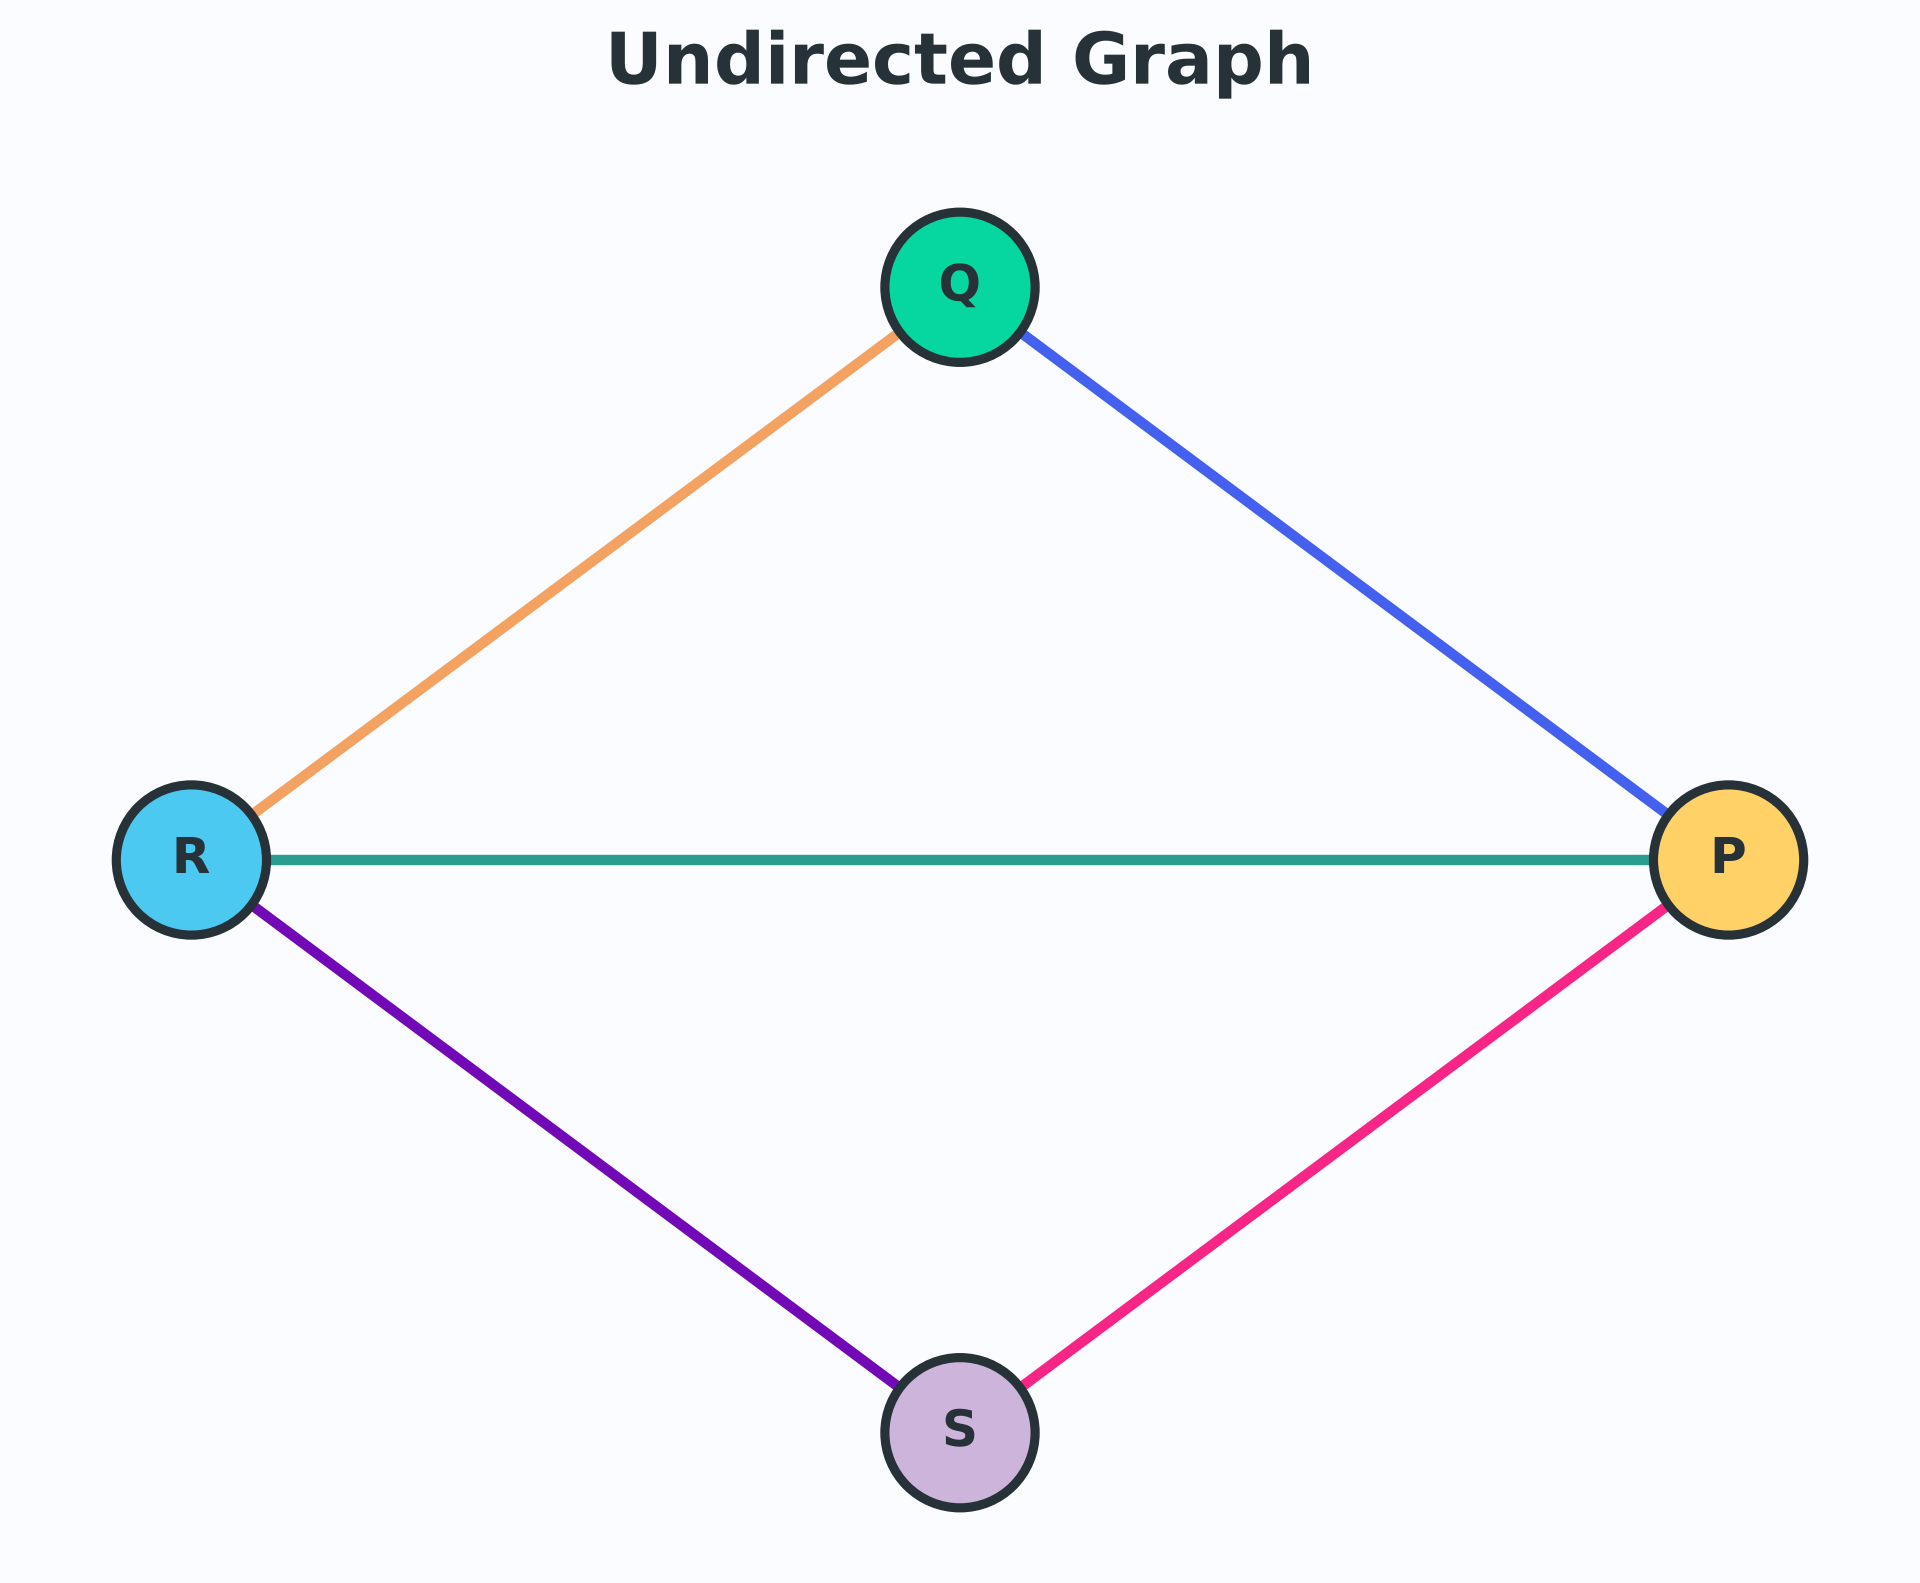
\includegraphics[width=\linewidth,height=4cm,keepaspectratio]
{graph_images/undirected_graph.png}
\end{minipage}

\vspace{0.35cm}

% 2.6 Weighted Graph
\subsection{Weighted Graph}

\noindent
\begin{minipage}[c]{0.58\textwidth}
A weighted graph is a graph in which numerical values,
called weights, are assigned to its edges. These
weights may represent distance, cost, time or capacity.
Weighted graphs are useful in transportation and
communication networks, where the shortest or least
expensive route needs to be identified.
\end{minipage}
\hfill
\begin{minipage}[c]{0.36\textwidth}
\centering
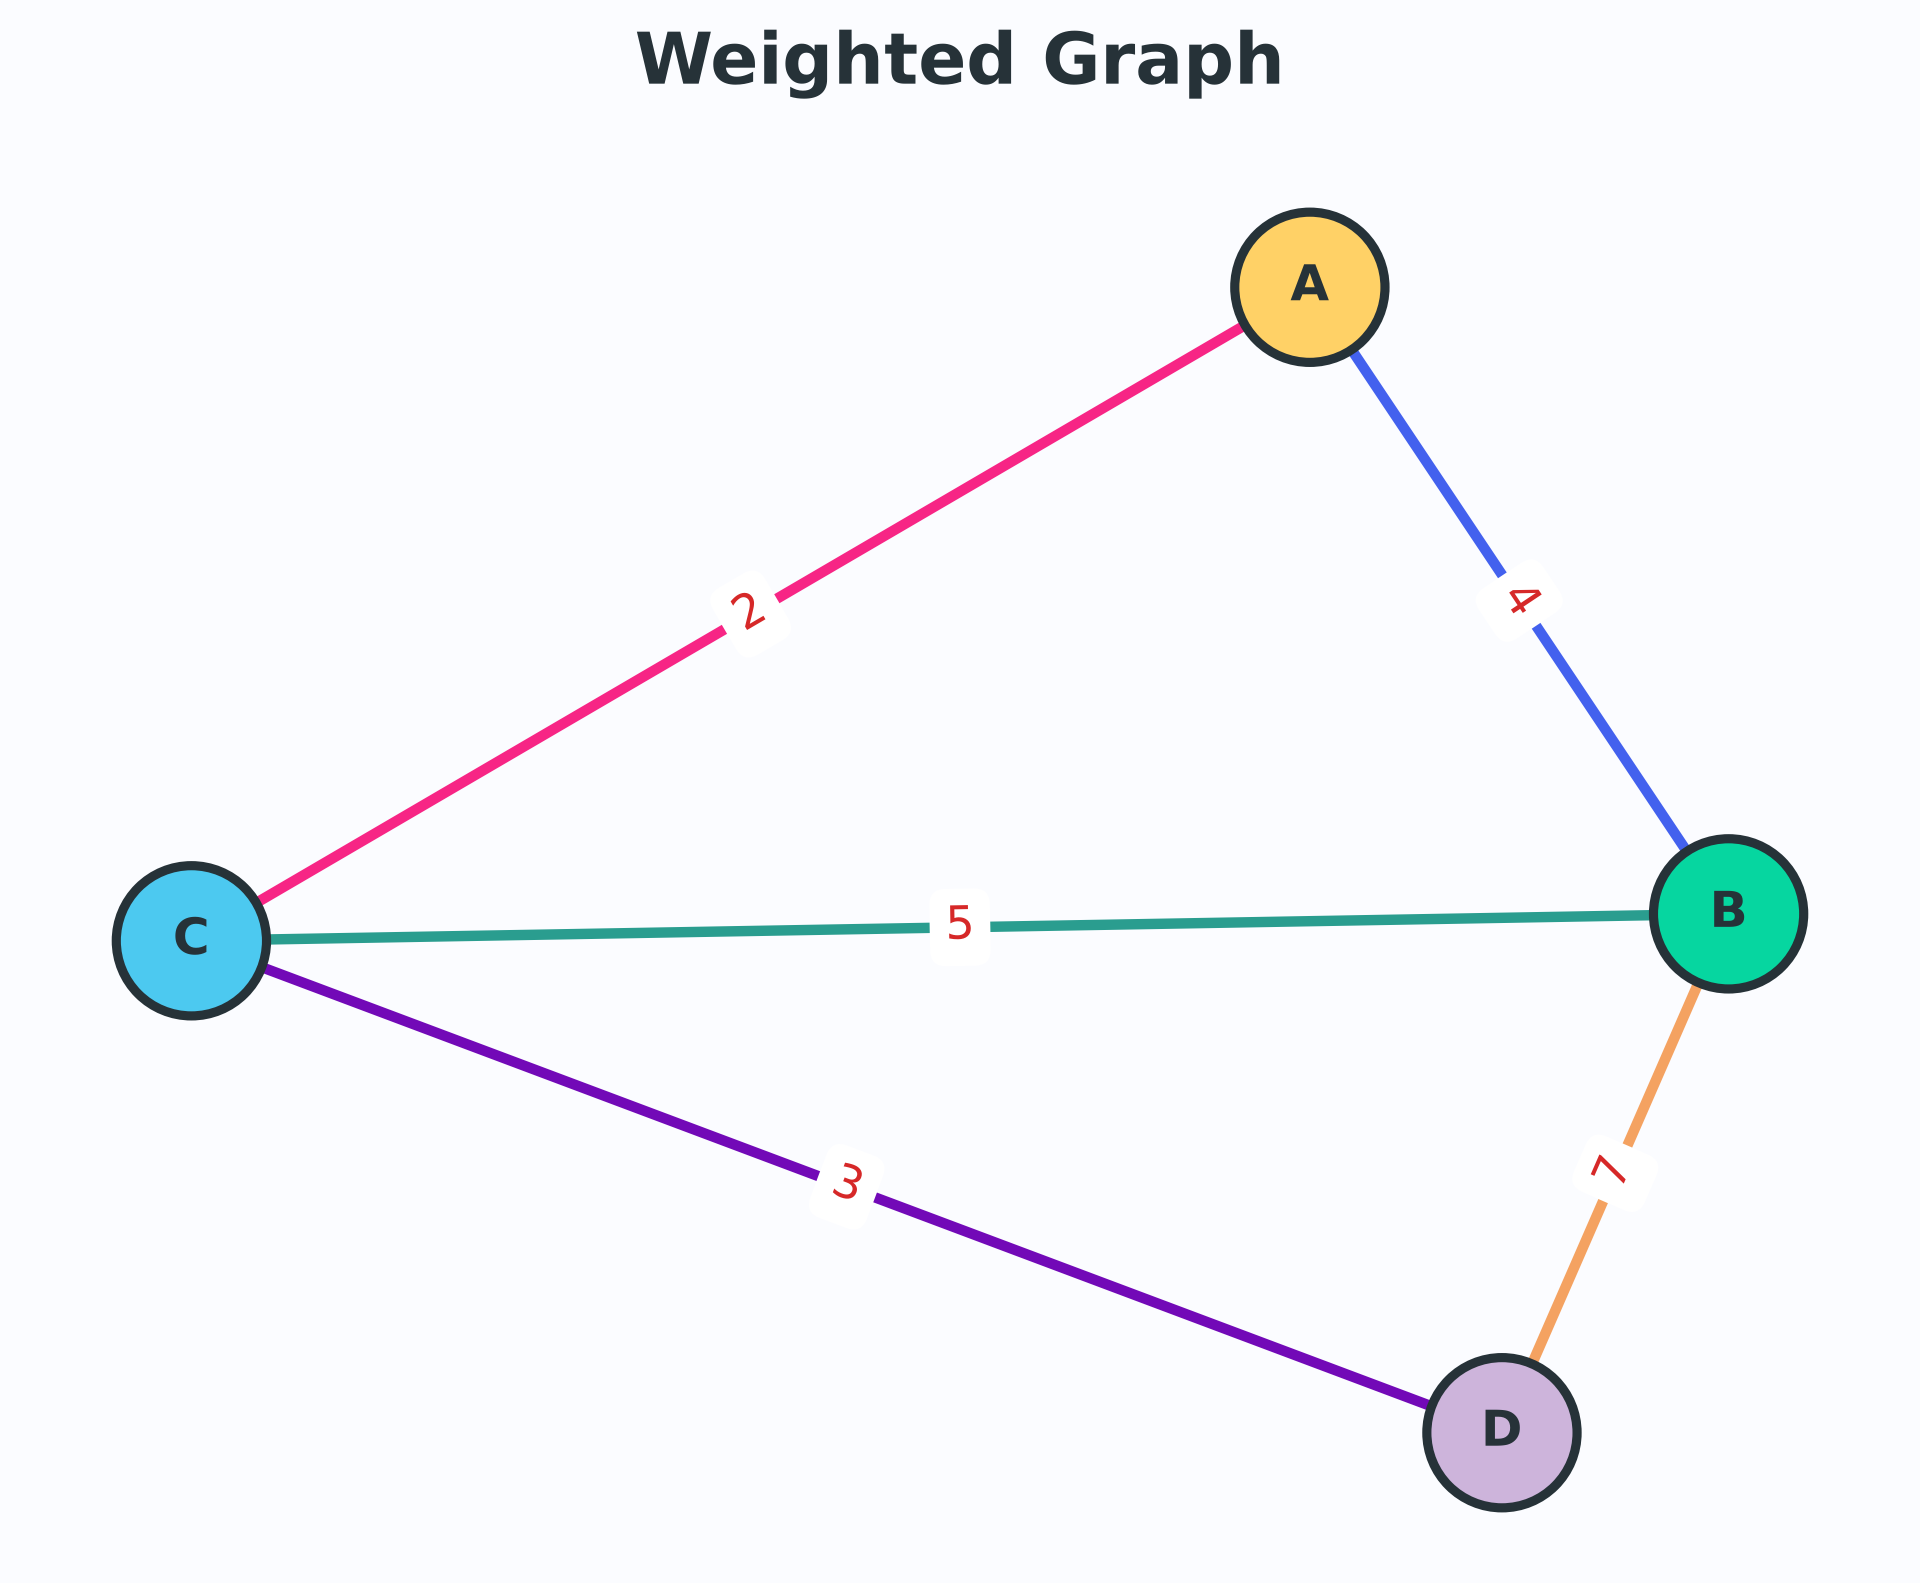
\includegraphics[width=\linewidth,height=4cm,keepaspectratio]
{graph_images/weighted_graph.png}
\end{minipage}

\vspace{0.35cm}

% 2.7 Mixed Graph
\subsection{Mixed Graph}

\noindent
\begin{minipage}[c]{0.58\textwidth}
A mixed graph contains both directed and undirected
edges. It is used to represent systems where some
relationships have a specific direction while others
do not. For example, a transportation network may
contain one-way roads and two-way roads represented
within the same graph.
\end{minipage}
\hfill
\begin{minipage}[c]{0.36\textwidth}
\centering
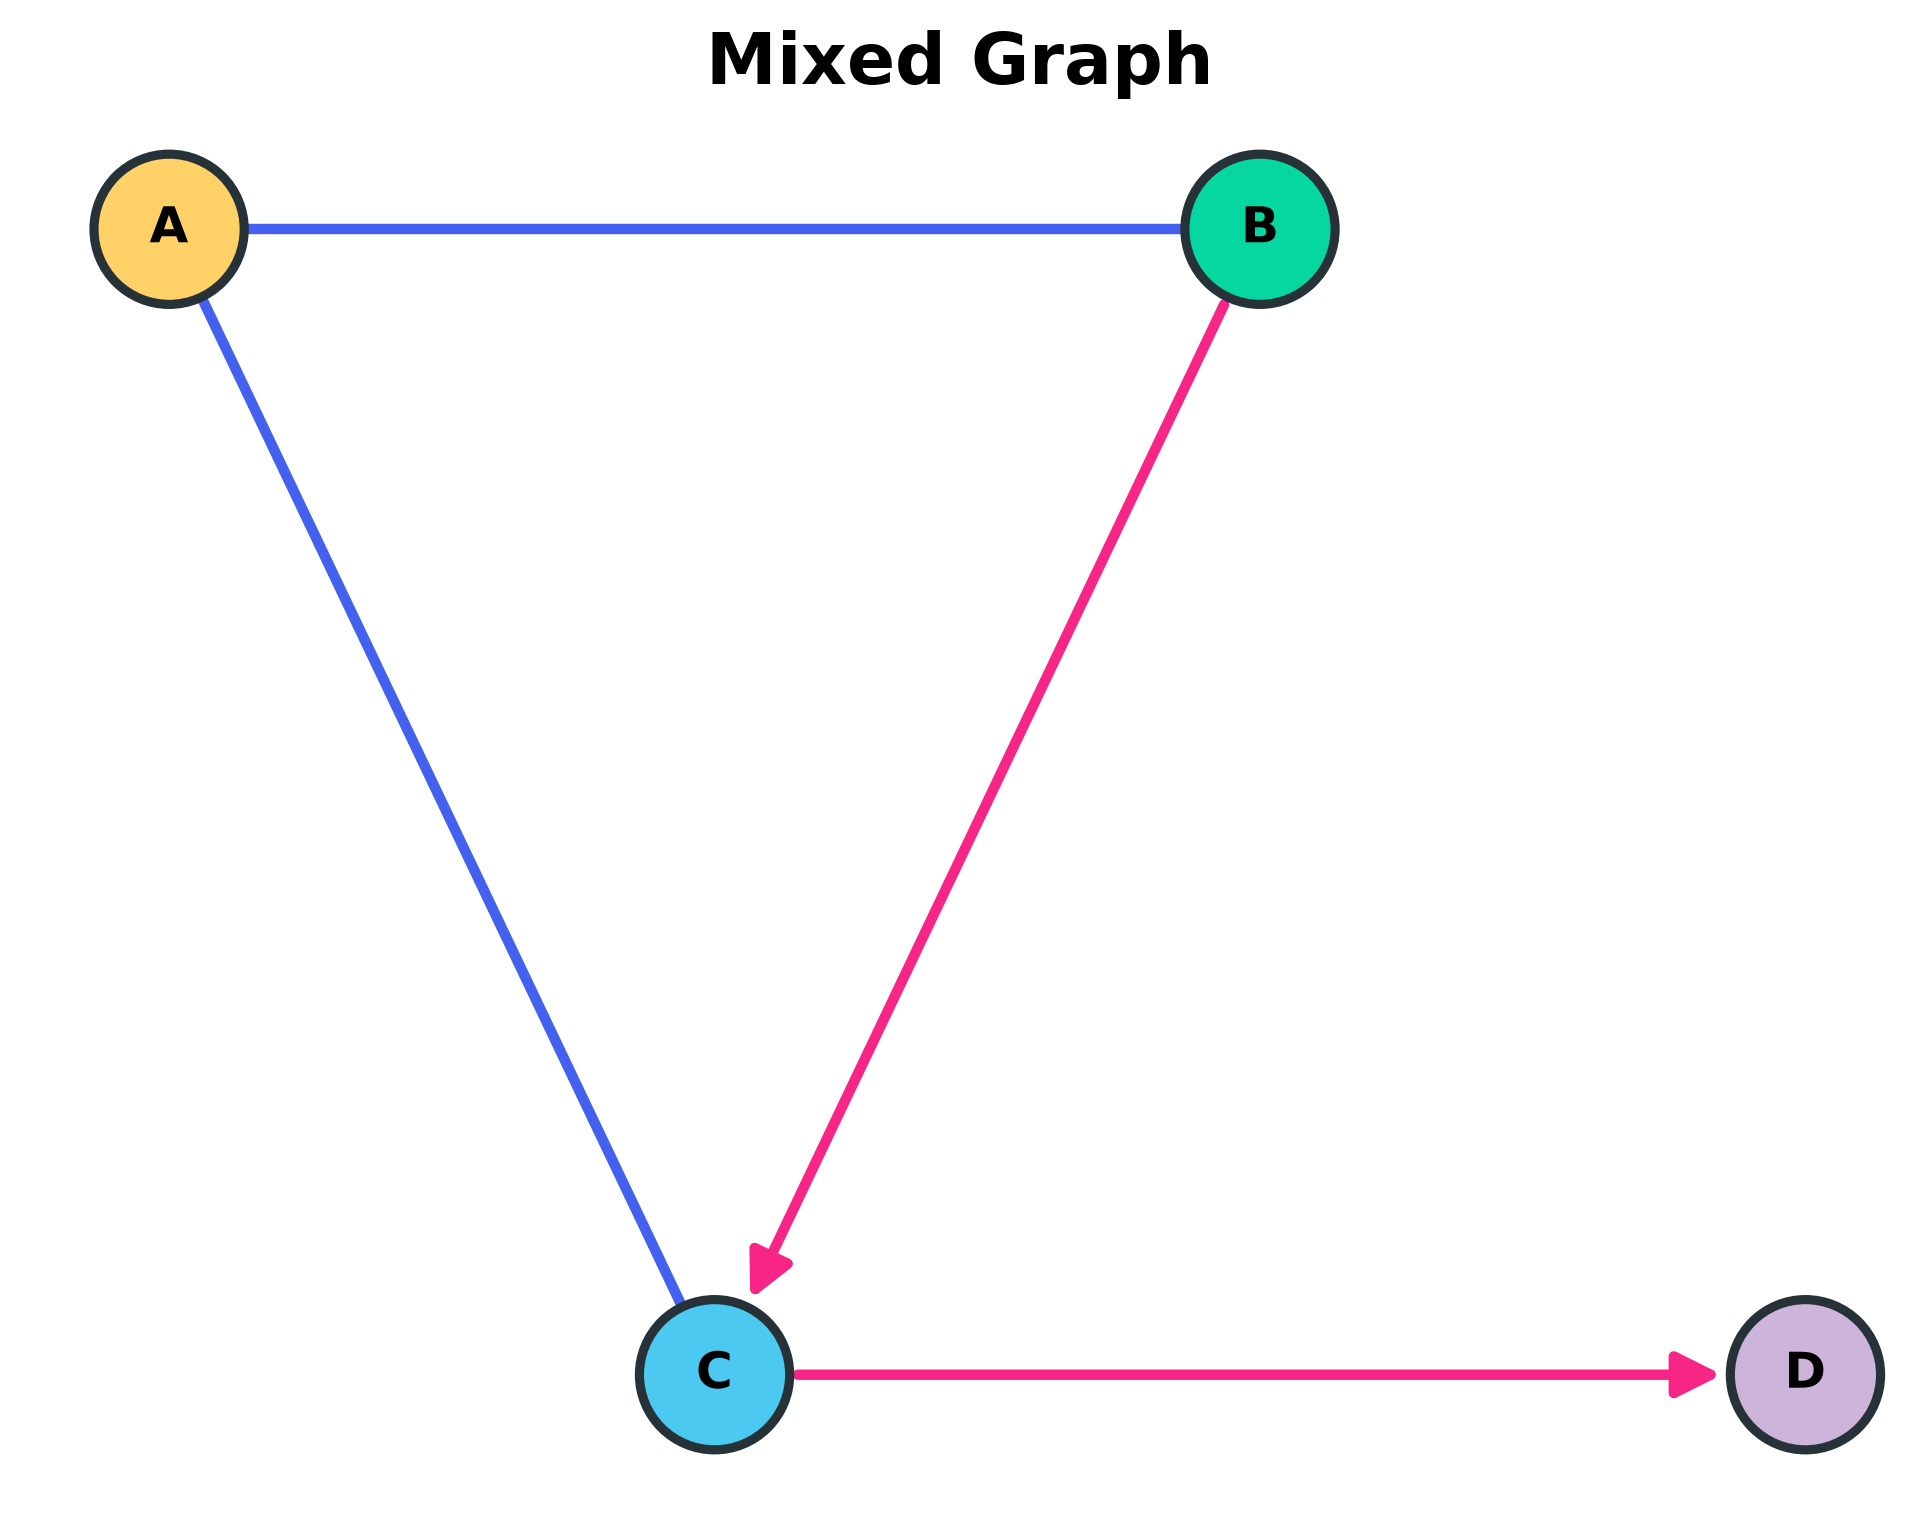
\includegraphics[width=\linewidth,height=4cm,keepaspectratio]
{graph_images/mixed_graph.png}
\end{minipage}



%================================================
% SECTION 3: SPECIAL GRAPHS
%================================================

\section{Special Graphs}

Special graphs are important categories of graphs that have specific
properties and structures. They are widely used in computer networks,
communication systems, scheduling, circuit design and data organisation.

\subsection{Complete Graph}

A complete graph is a simple graph in which every pair of distinct
vertices is connected by an edge. It is represented by $K_n$,
where $n$ is the number of vertices.

The number of edges in a complete graph is:

\[
|E(K_n)| = \frac{n(n-1)}{2}
\]

The degree of every vertex is:

\[
\deg(v)=n-1
\]

For example, $K_5$ contains five vertices and ten edges.

\begin{figure}[htbp]
    \centering
    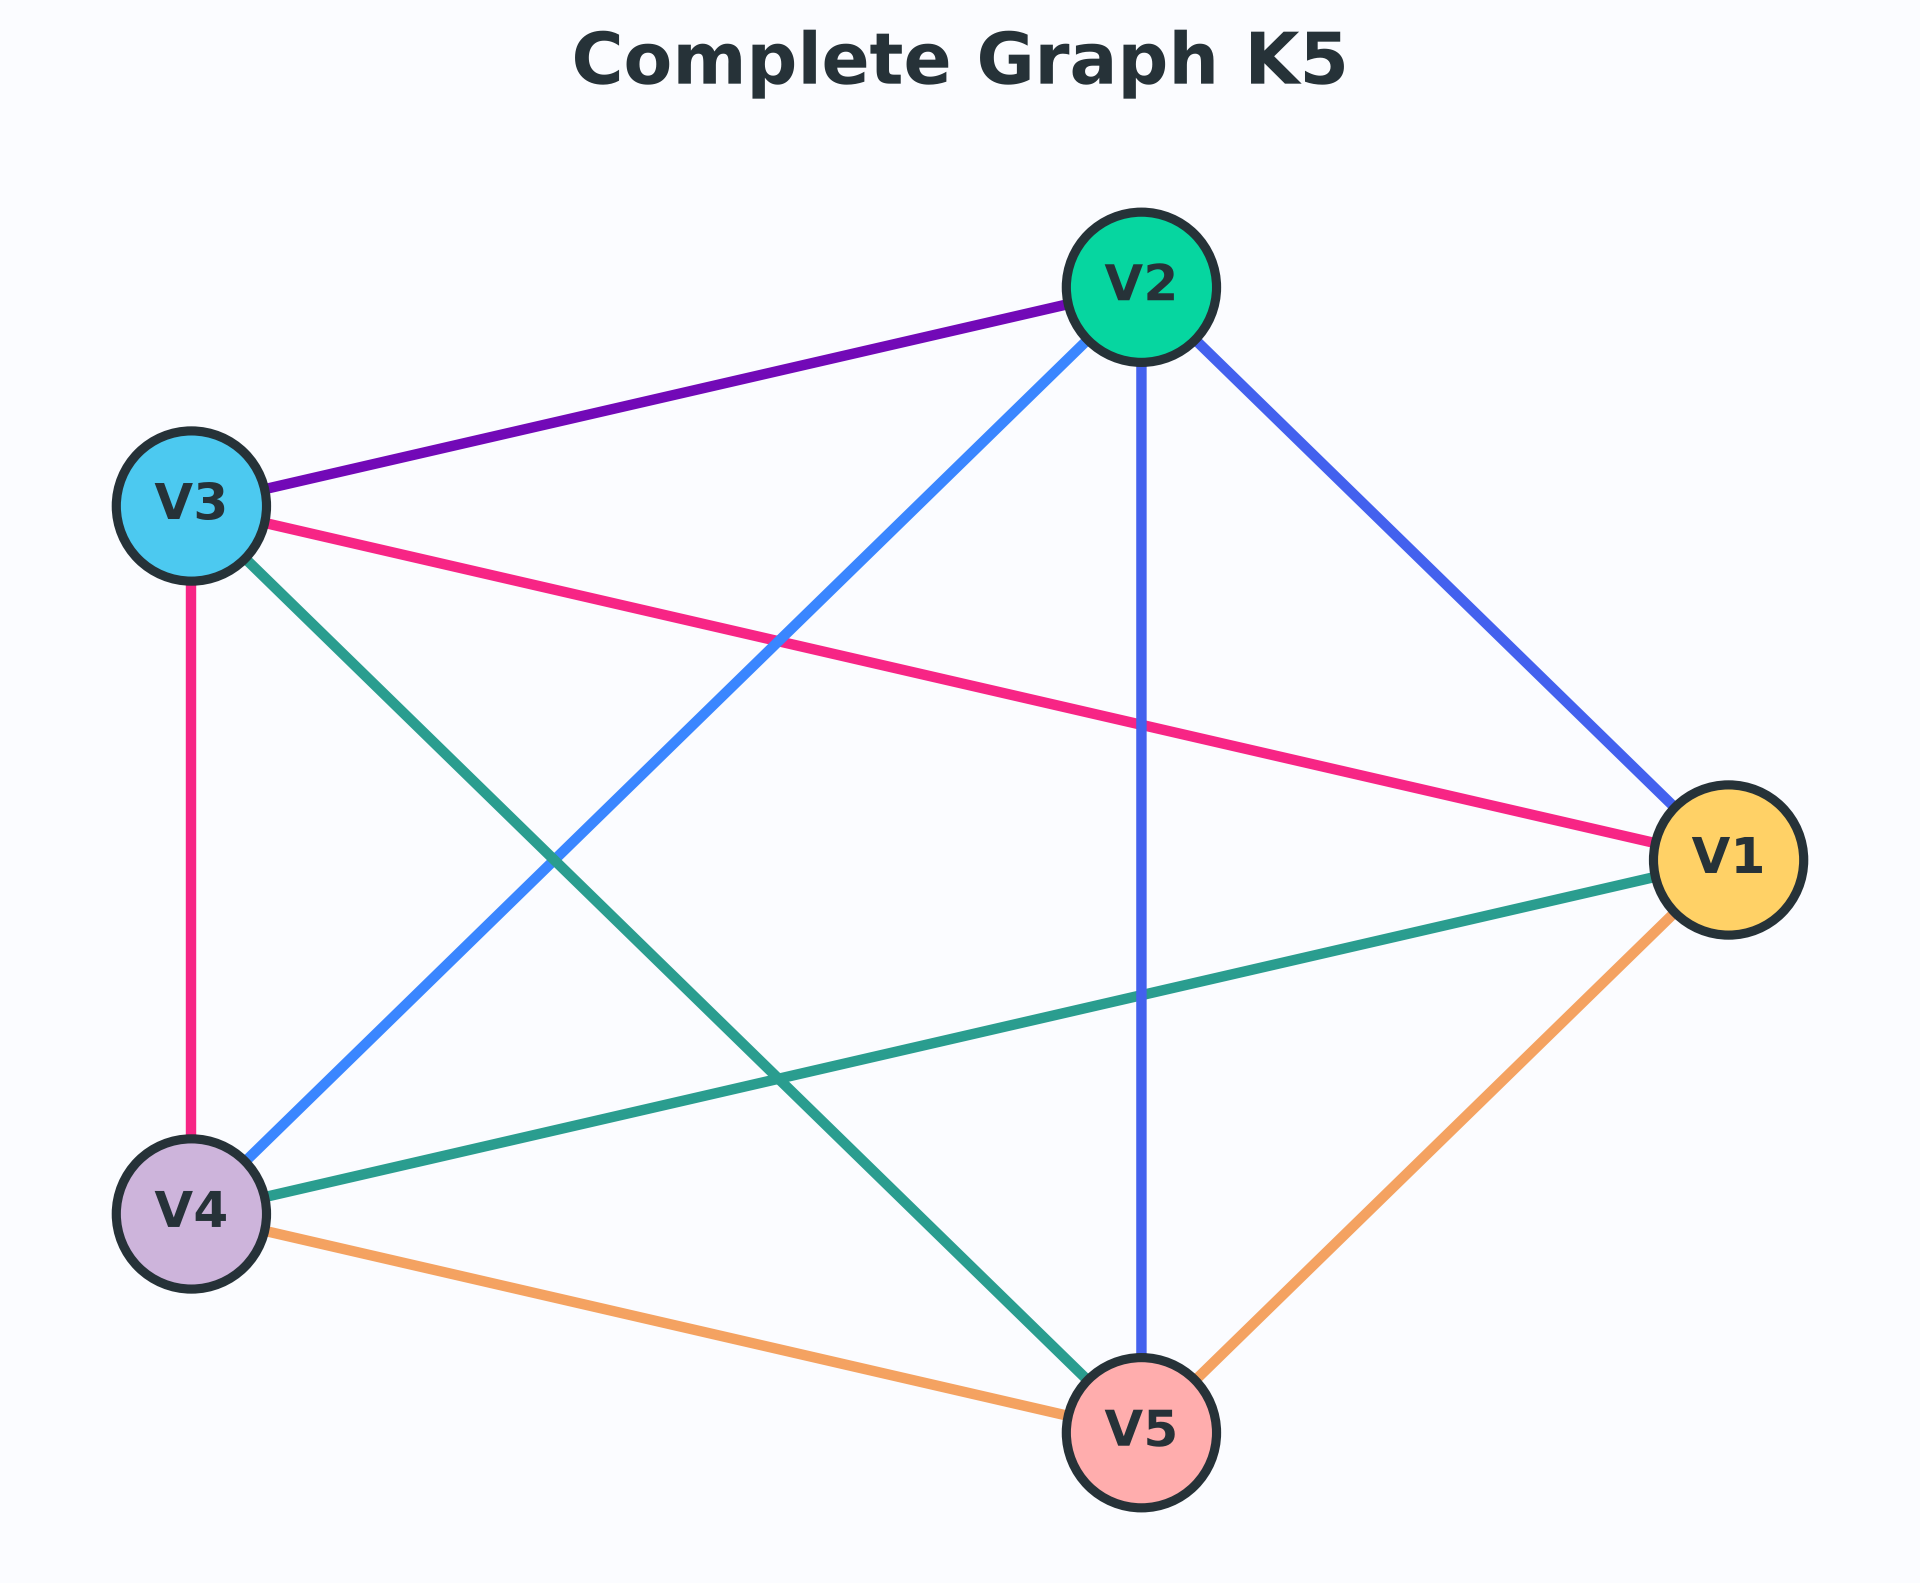
\includegraphics[width=0.40\textwidth]
    {graph_images/complete_graph.png}
    \label{fig:complete-graph}
\end{figure}

\textbf{Practical Application:}
Complete graphs represent fully connected communication networks
where every device can directly communicate with every other device.
However, the number of connections increases rapidly as the number
of devices grows.

\subsection{Bipartite Graph}

A bipartite graph is a graph whose vertex set can be divided into
two disjoint sets, such that every edge connects a vertex from one
set to a vertex in the other set.

A complete bipartite graph is represented by $K_{m,n}$.

The number of edges is:

\[
|E(K_{m,n})|=mn
\]

A graph is bipartite if and only if it contains no cycle of odd length.

\begin{figure}[htbp]
    \centering
    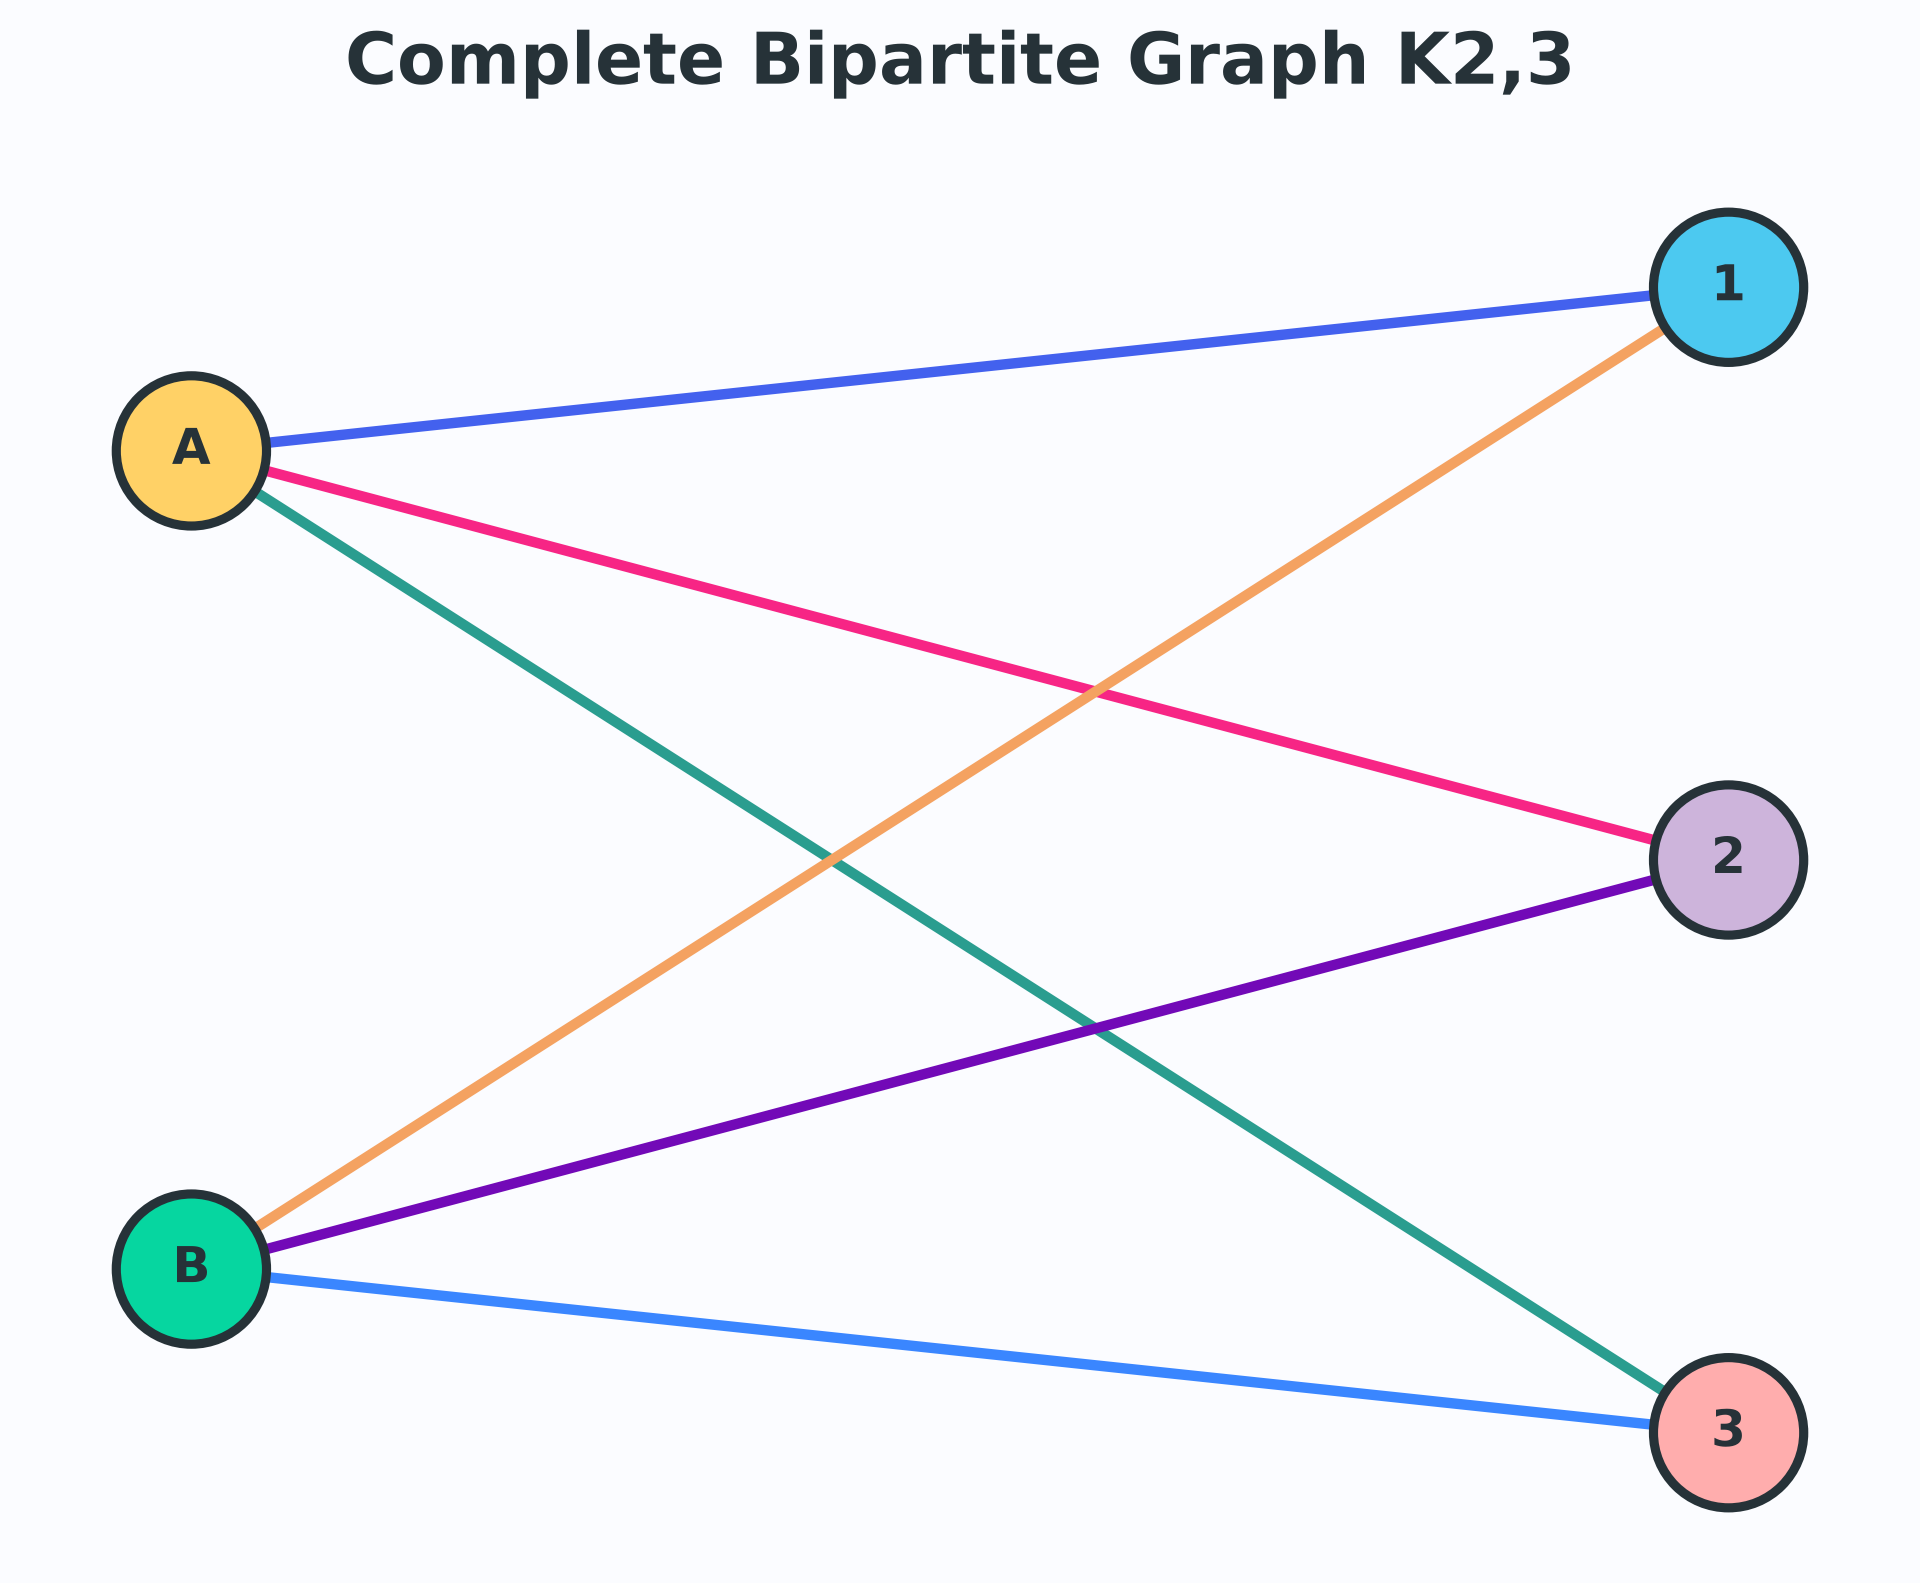
\includegraphics[width=0.40\textwidth]
    {graph_images/bipartite_graph.png}
    \label{fig:bipartite-graph}
\end{figure}

\textbf{Practical Application:}
Bipartite graphs are used in job allocation systems, student-course
assignments and matching problems. For example, students can be
connected to the courses they have selected.

\subsection{Regular Graph}

A regular graph is a graph in which every vertex has the same degree.
If every vertex has degree $k$, the graph is called a $k$-regular graph.

The number of edges in a $k$-regular graph with $n$ vertices is:

\[
|E|=\frac{nk}{2}
\]

For example, a cycle graph with six vertices is a 2-regular graph,
because every vertex has exactly two edges.

\begin{figure}[htbp]
    \centering
    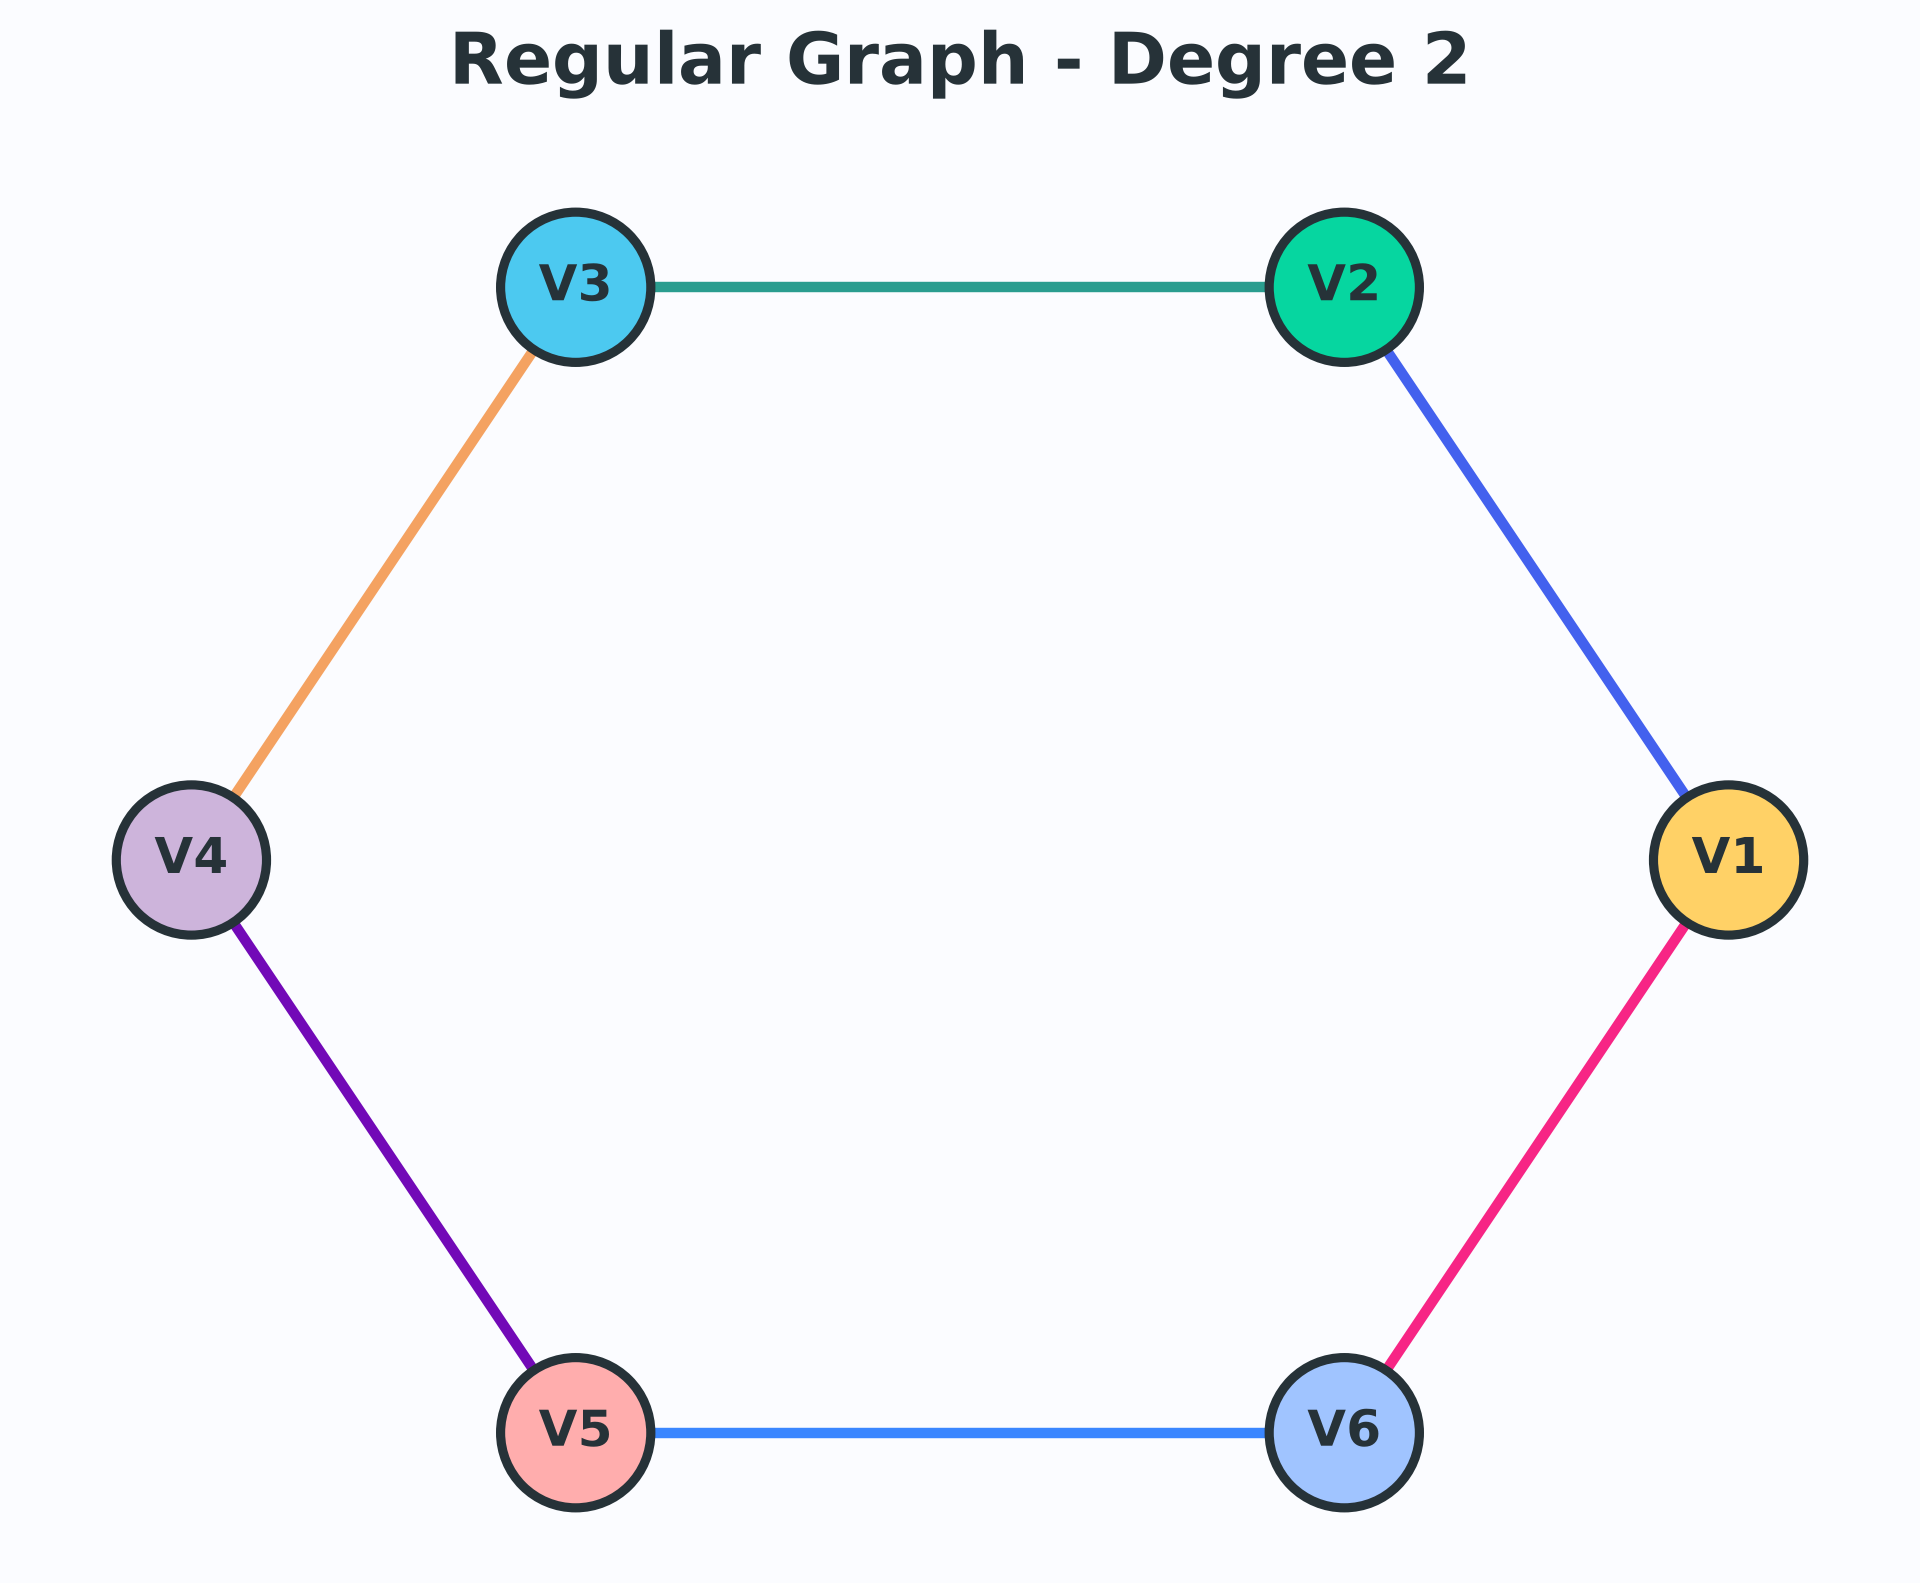
\includegraphics[width=0.40\textwidth]
    {graph_images/regular_graph.png}
    \label{fig:regular-graph}
\end{figure}

\textbf{Practical Application:}
Regular graphs are used in network topology design. They help
distribute connections evenly among network devices, supporting
balanced communication and load distribution.

\subsection{Tree}

A tree is a connected undirected graph that contains no cycles.
It is commonly used to represent hierarchical relationships.

A tree with $n$ vertices always contains:

\[
|E|=n-1
\]

Some important properties of trees are:
\begin{itemize}
    \item A tree is connected and acyclic.
    \item There is exactly one path between every pair of vertices.
    \item A tree with at least two vertices has at least two leaves.
    \item Removing any edge disconnects the tree.
\end{itemize}

\begin{figure}[htbp]
    \centering
    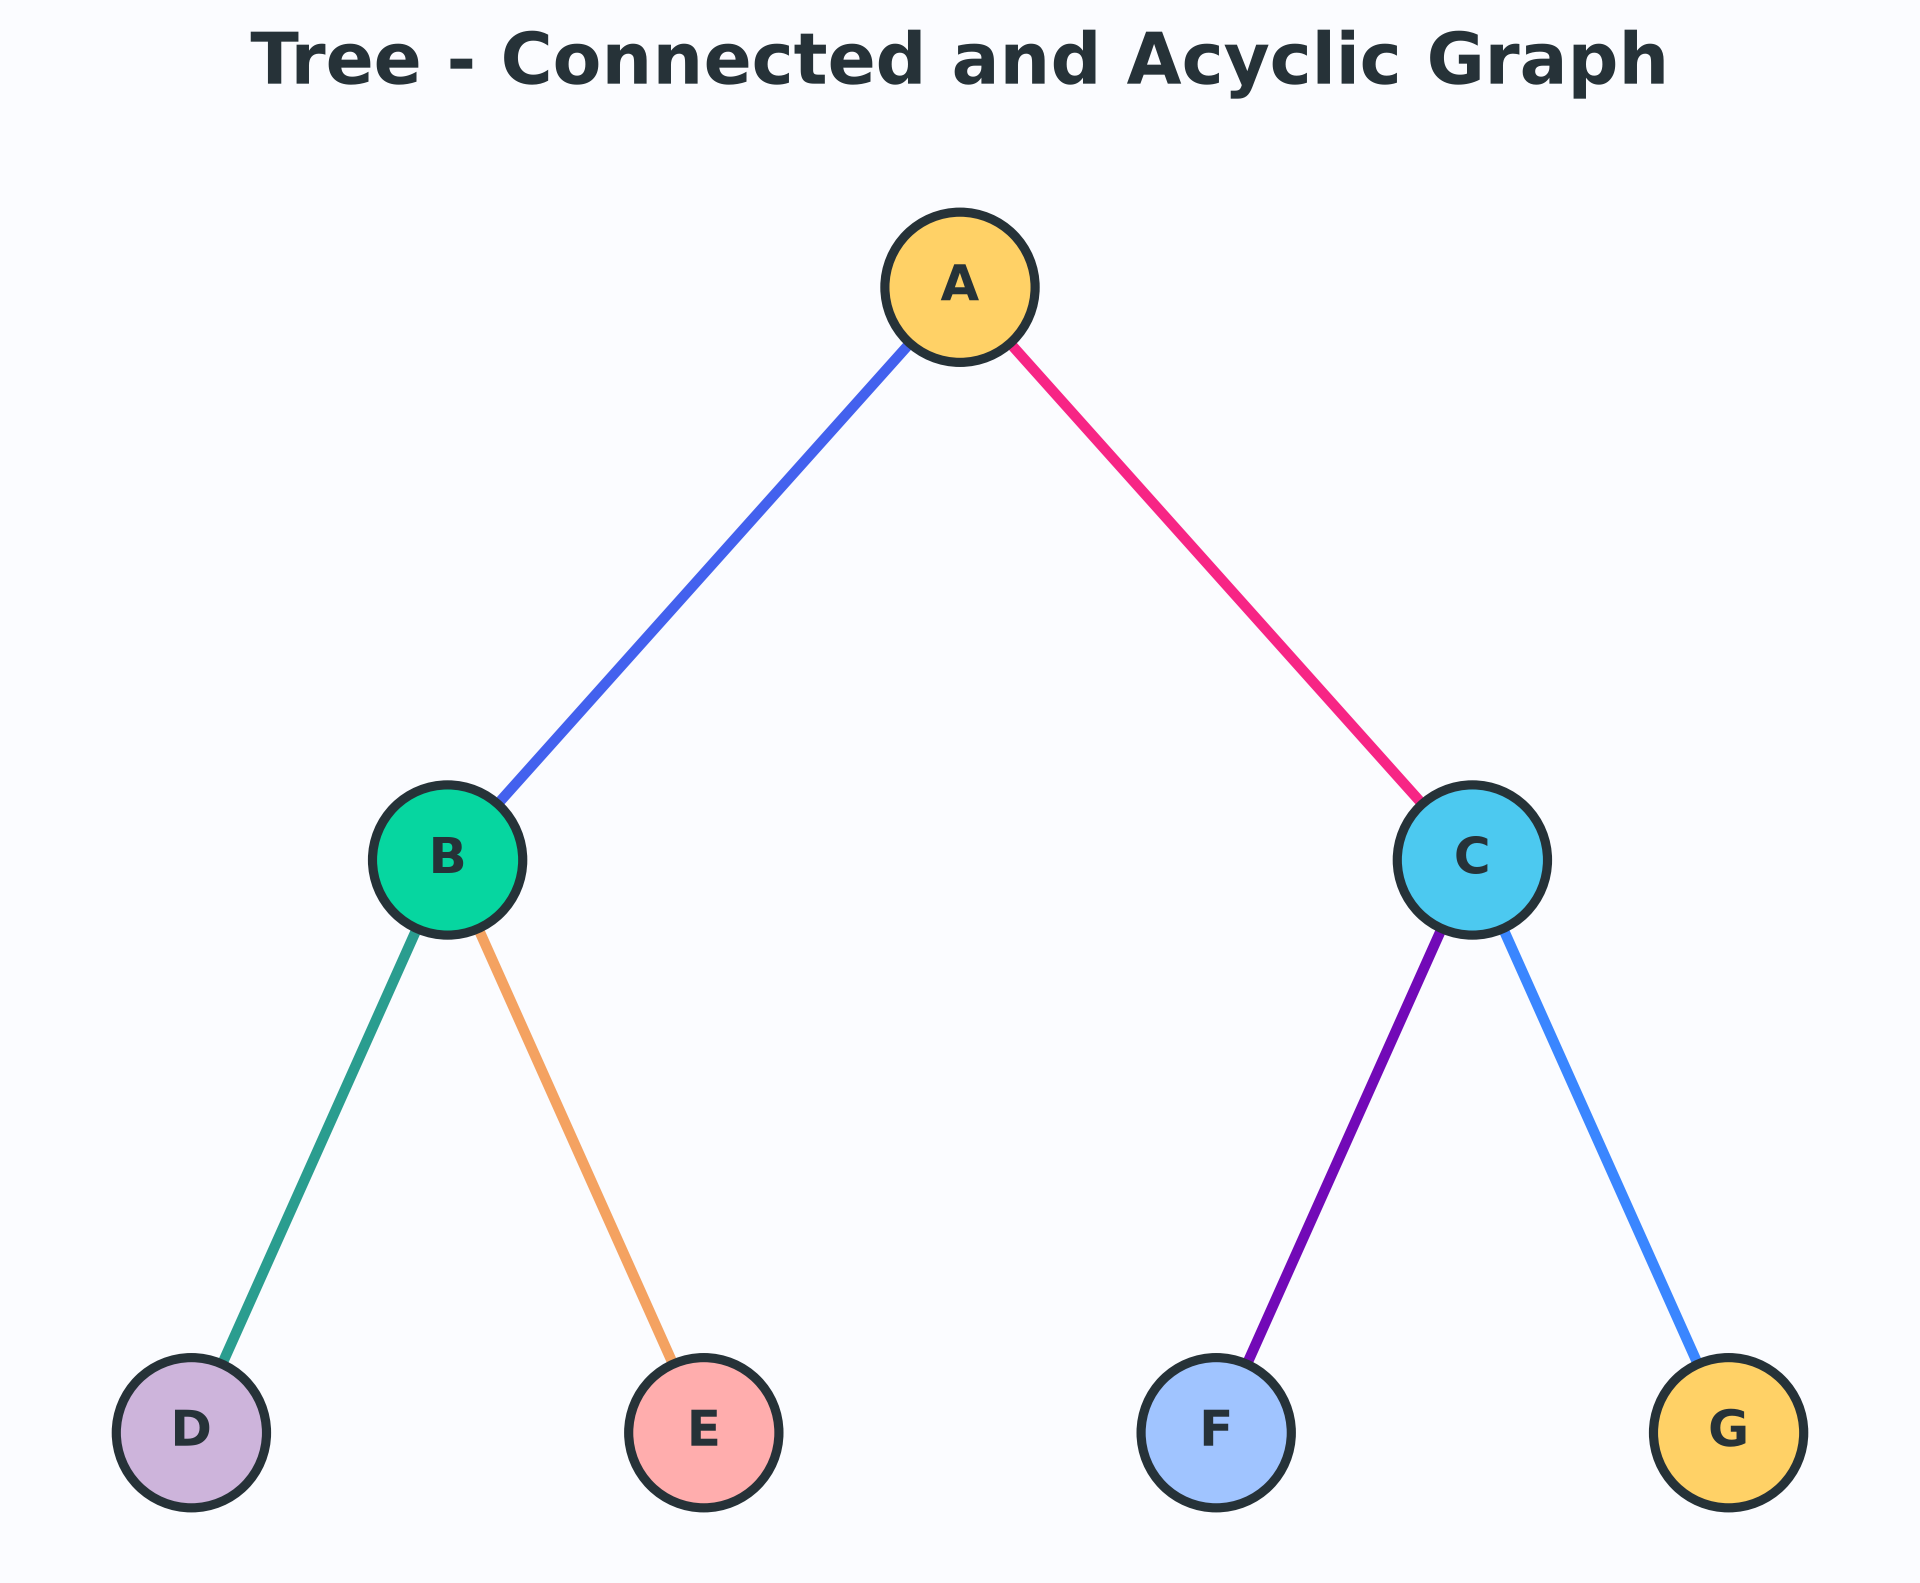
\includegraphics[width=0.40\textwidth]
    {graph_images/tree.png}
    \label{fig:tree}
\end{figure}

\textbf{Practical Application:}
Trees are used in file systems, organisation charts, database
indexing and decision-making structures. A computer's folder
structure is a common example of a tree.

\subsection{Planar Graph}

A planar graph is a graph that can be drawn on a plane without
any edges crossing each other, except at their common vertices.

For a connected planar graph, Euler's formula is:

\[
V-E+F=2
\]

where:
\begin{itemize}
    \item $V$ represents the number of vertices.
    \item $E$ represents the number of edges.
    \item $F$ represents the number of faces or regions.
\end{itemize}

For a simple connected planar graph with $V\geq 3$:

\[
E\leq 3V-6
\]

\begin{figure}[htbp]
    \centering
    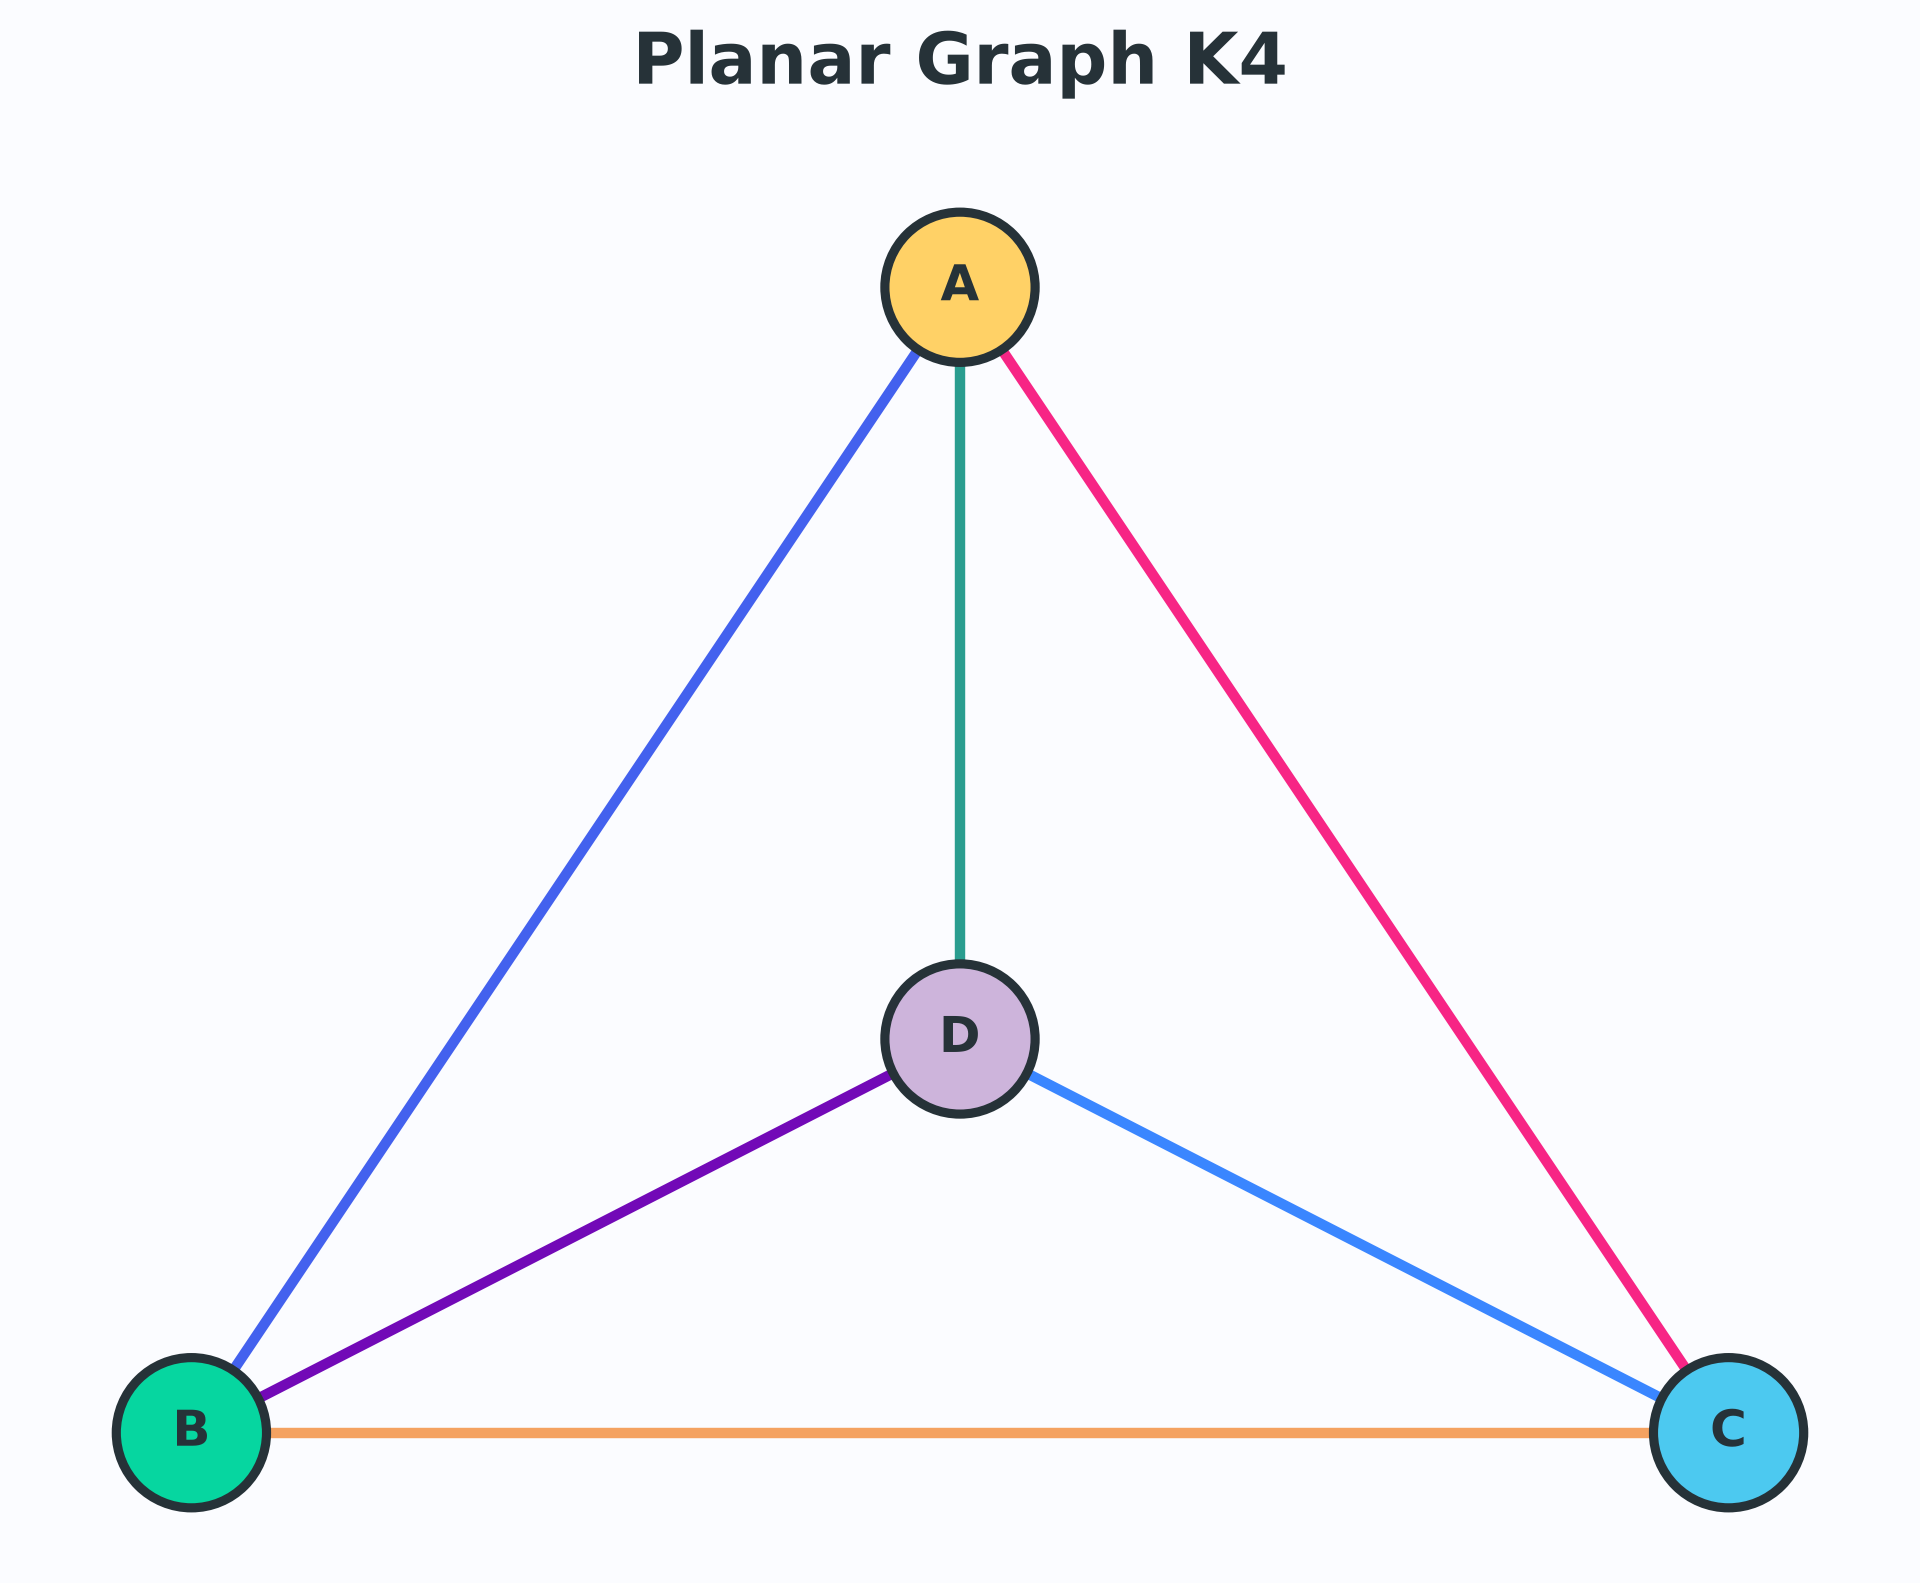
\includegraphics[width=0.35\textwidth]
    {graph_images/planar_graph.png}
    \label{fig:planar-graph}
\end{figure}

\textbf{Practical Application:}
Planar graphs are useful in printed circuit board design, road
network layouts and geographical map representation, where
crossing connections must be minimised or avoided.

\subsection{Eulerian Graph}

An Eulerian graph is a connected graph that contains an Euler circuit.
An Euler circuit is a closed trail that traverses every edge exactly
once and returns to its starting vertex.

A connected graph is Eulerian if every vertex has an even degree.

\begin{figure}[htbp]
    \centering
    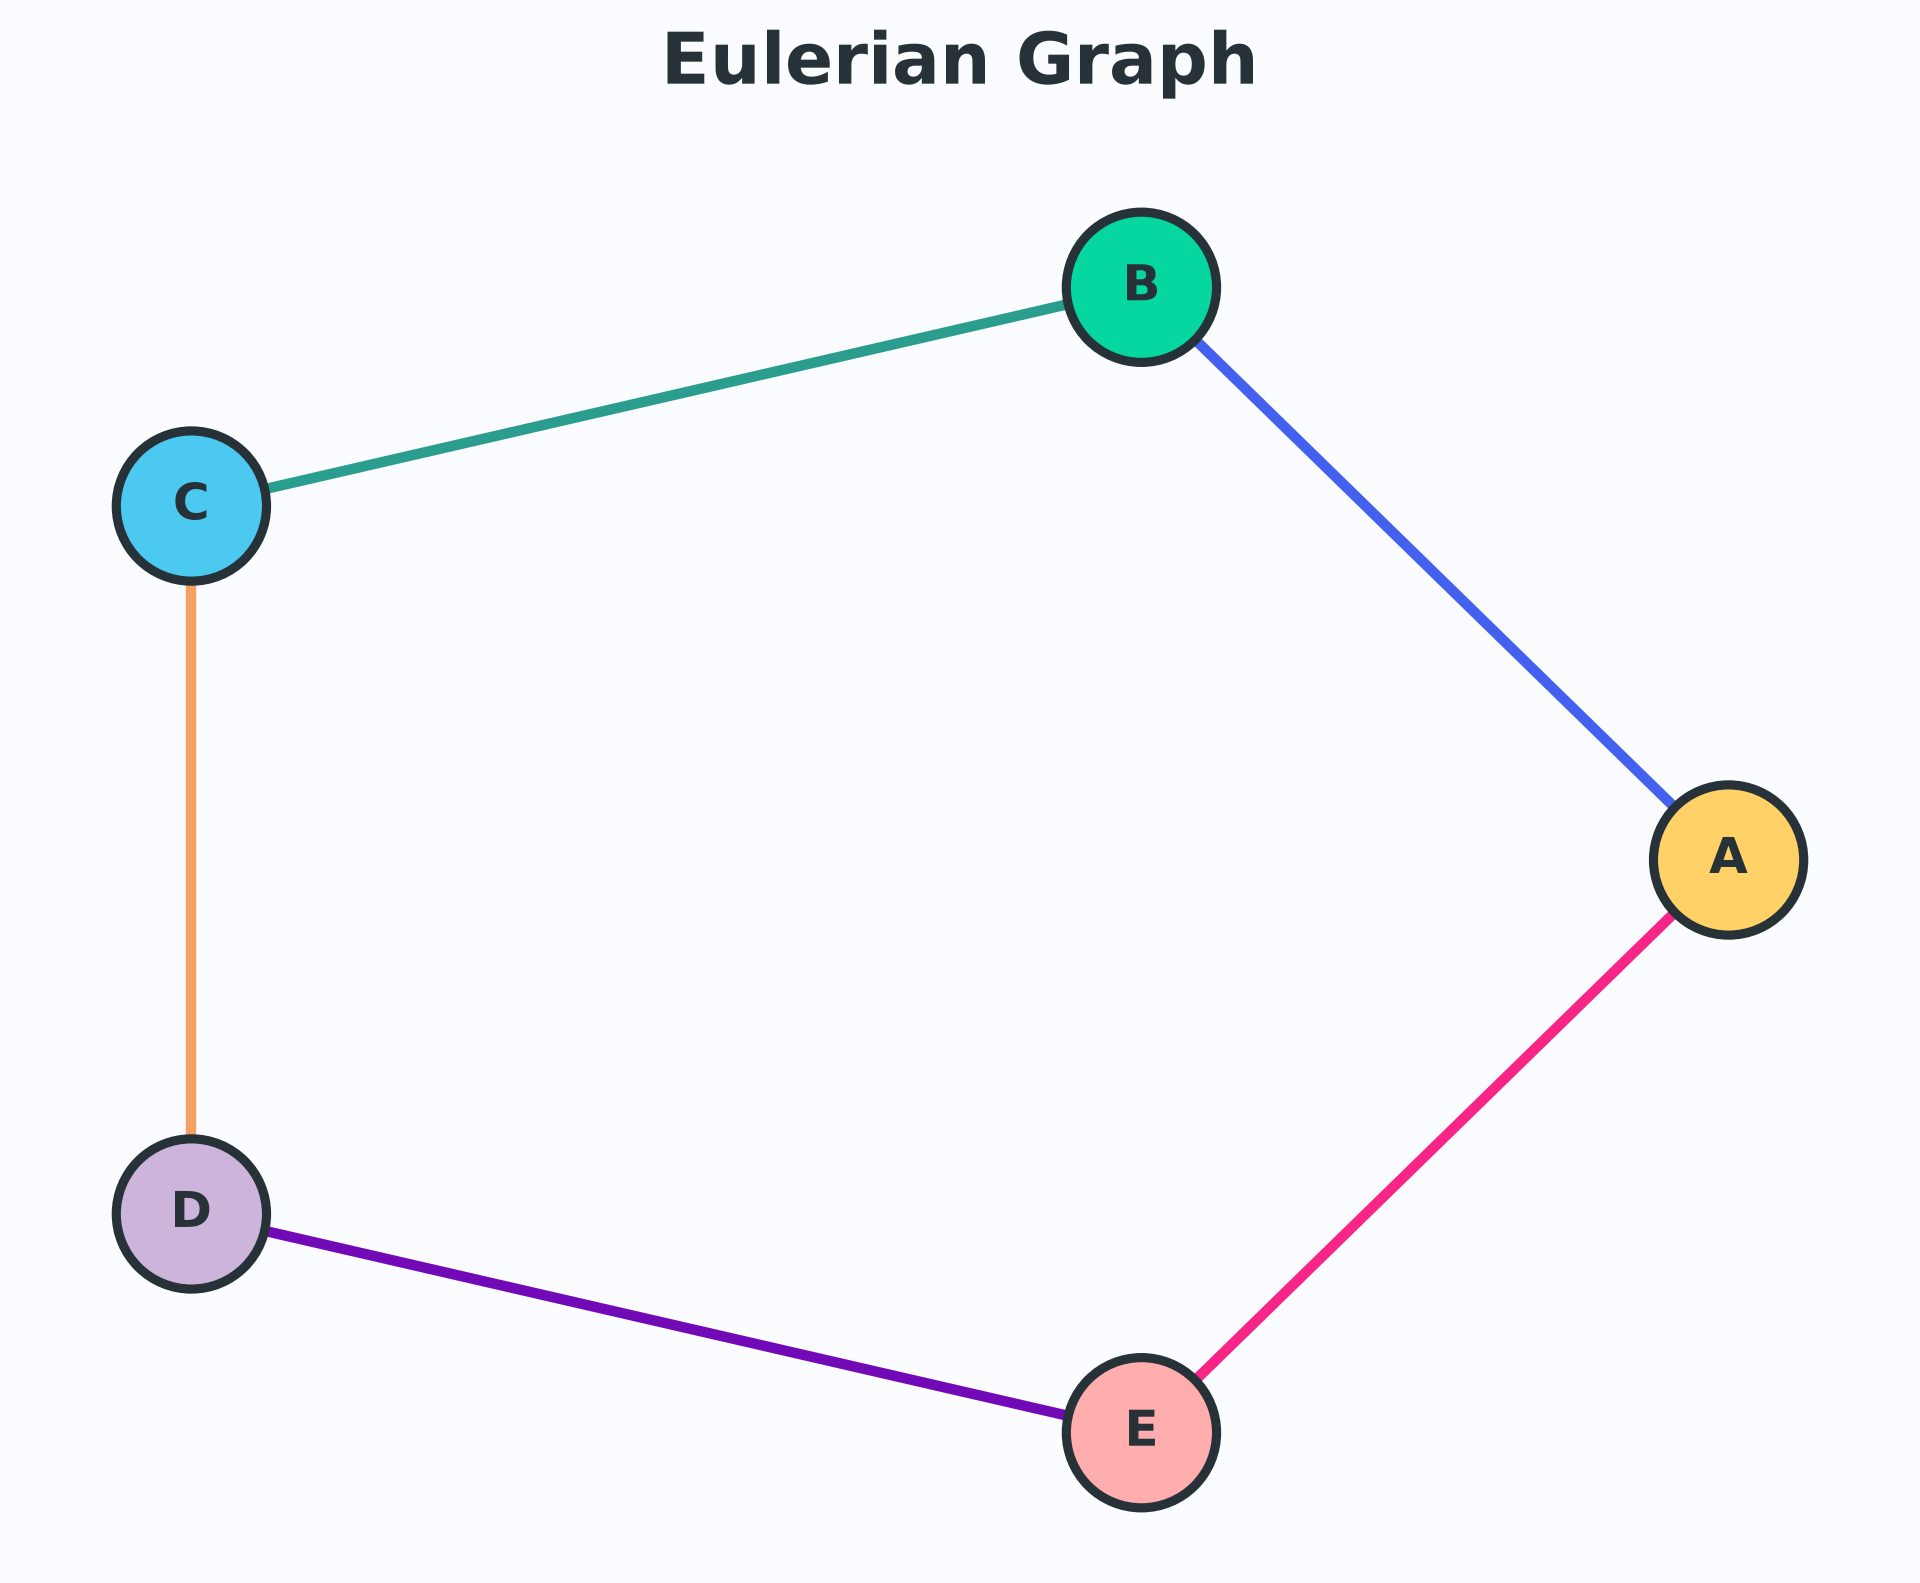
\includegraphics[width=0.40\textwidth]
    {graph_images/eulerian_graph.png}
    \label{fig:eulerian-graph}
\end{figure}

\textbf{Practical Application:}
Eulerian graphs are useful in route planning, street sweeping,
postal delivery and inspection systems, where every road or
connection must be covered.

\subsection{Hamiltonian Graph}

A Hamiltonian graph is a graph that contains a Hamiltonian cycle.
A Hamiltonian cycle visits every vertex exactly once and returns
to the starting vertex.

Unlike an Euler circuit, which focuses on visiting every edge,
a Hamiltonian cycle focuses on visiting every vertex.

\begin{figure}[htbp]
    \centering
    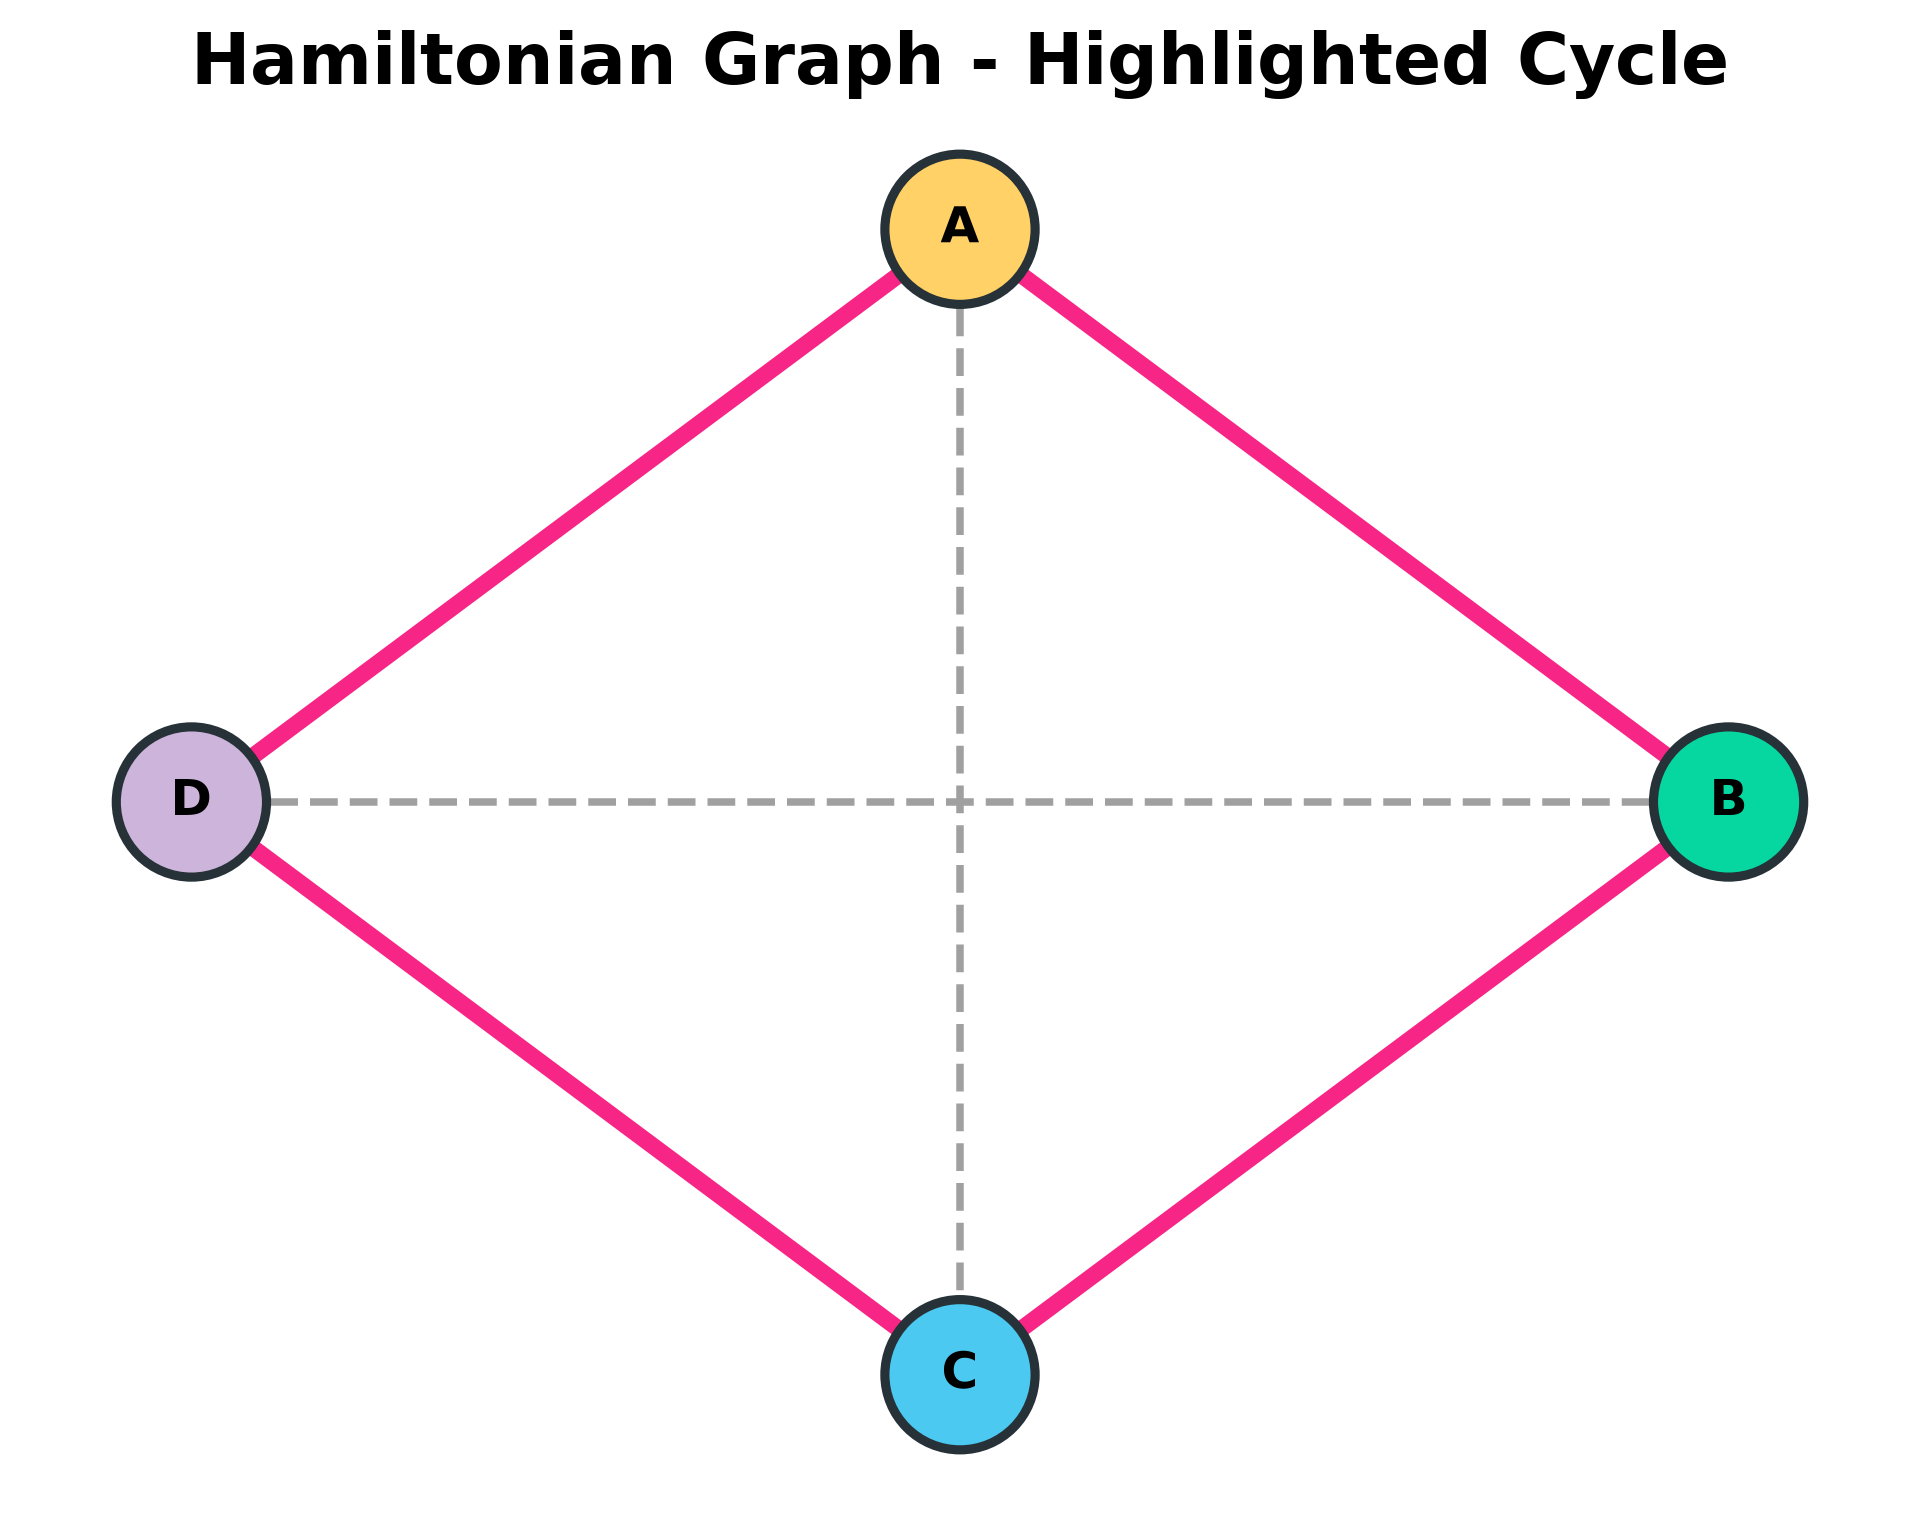
\includegraphics[width=0.40\textwidth]
    {graph_images/hamiltonian_graph.png}
    \label{fig:hamiltonian-graph}
\end{figure}

\textbf{Practical Application:}
Hamiltonian graphs are related to travelling salesperson problems,
delivery route planning and logistics, where a route must visit
each location once before returning to the starting point.

\subsection{Summary of Special Graphs}

\begin{table}[htbp]
\centering
\caption{Comparison of Special Graphs}
\label{tab:special-graphs}
\renewcommand{\arraystretch}{1.4}
\begin{tabular}{|p{3cm}|p{7cm}|p{5cm}|}
\hline
\textbf{Graph Type} & \textbf{Main Property} & \textbf{Application} \\
\hline
Complete Graph & Every pair of vertices is adjacent & Fully connected networks \\
\hline
Bipartite Graph & Vertices divided into two disjoint sets & Job and student allocation \\
\hline
Regular Graph & Every vertex has equal degree & Network topology \\
\hline
Tree & Connected graph without cycles & File systems and hierarchies \\
\hline
Planar Graph & Can be drawn without edge crossings & Circuit and road layouts \\
\hline
Eulerian Graph & Every edge is traversed exactly once in a circuit & Route inspection \\
\hline
Hamiltonian Graph & Every vertex is visited exactly once in a cycle & Delivery route planning \\
\hline
\end{tabular}
\end{table}

%================================================
% SECTION 6: PRACTICAL APPLICATIONS OF GRAPH THEORY
%================================================

\section{Practical Applications of Graph Theory}

Graph theory has many practical applications in computer science,
engineering, communication and everyday life. It provides a
mathematical method for representing relationships between
different objects and analysing how they are connected. By
representing objects as vertices and their relationships as
edges, complex systems can be studied and managed more
efficiently. Some important applications of graph theory are
discussed below.

\subsection{Computer Networks and Communication Systems}

Graph theory is widely used in computer networks to represent
connections between computers, routers and servers. In this
representation, each device is considered a vertex, while the
communication links between devices are represented by edges.
Weighted graphs can represent factors such as transmission
cost, distance, capacity and network latency. Graph algorithms
help identify routes between devices and analyse network
connectivity. For example, routing systems use graph-based
methods to determine suitable paths for transferring data
between different locations.

\subsection{Social Networks and Recommendation Systems}

Social networking platforms can be represented using graphs
in which users are vertices and relationships such as friendships
or follows are edges. Graph analysis helps identify highly
connected users, communities and relationships between
different groups. Platforms such as LinkedIn use network
relationships to suggest people that users may know. Similarly,
recommendation systems represent users and items using
bipartite graphs. These connections can be analysed to identify
possible interests and recommend relevant content or products.

\subsection{Transportation and Route Planning}

Graph theory is useful in transportation systems because roads,
stations and locations can be represented as vertices and the
routes connecting them as edges. In weighted graphs, the edges
can represent distance, travel time or transportation cost.
Shortest-path algorithms help identify efficient routes between
locations. Eulerian graph concepts are also useful in route
inspection problems, where every road or connection must be
covered. These applications are important in navigation,
delivery services, public transportation and logistics.

\subsection{Examination Timetabling and Scheduling}

Graph colouring is used to solve scheduling problems in which
conflicting activities should not be assigned to the same time
slot. In examination timetabling, each examination is represented
as a vertex, and an edge is created between two examinations
if some students are enrolled in both. Different colours represent
different examination time slots. A proper colouring ensures
that no two connected examinations are scheduled at the same
time. The chromatic number represents the minimum number
of colours required for a proper colouring. This approach helps
educational institutions prepare examination timetables without
clashes.



\subsection{Database Systems and Knowledge Graphs}

Graph structures are used in graph databases and knowledge
representation systems to store relationships between different
entities. In a knowledge graph, objects such as people, places,
organisations and concepts are represented as vertices, while
their relationships are represented as edges. Graph databases
such as Neo4j store and retrieve connected information through
graph traversal. This approach is useful when information
contains complex relationships because related data can be
explored through connections rather than relying only on
multiple table joins.


%================================================
% SECTION 8: CONCLUSION AND FUTURE SCOPE
%================================================

\section{Conclusion}

Graph theory is an important branch of discrete mathematics
that deals with the study of vertices and edges and the
relationships between them. Different types of graphs, such
as simple graphs, directed graphs, weighted graphs, complete
graphs, bipartite graphs and trees, help represent various
real-world systems. The study of graph properties, including
degree, connectivity, paths and cycles, provides a mathematical
approach to understanding network structures.

Graph visualization makes these concepts easier to understand
by presenting vertices and edges in a graphical form. Tools
such as Python, NetworkX, Matplotlib and Gephi help construct,
visualize and analyse graphs. Algorithms such as Breadth-First
Search and Depth-First Search are useful for exploring graph
structures and finding connections between vertices.

Graph theory has practical applications in computer networks,
social media, transportation, examination scheduling, job
allocation and computer science. Therefore, it provides a
strong mathematical foundation for solving problems involving
relationships, connections and network structures.

%================================================
% SECTION 9: REFERENCES
%================================================

\section{References}

\begin{enumerate}

\item Kenneth H. Rosen, \textit{Discrete Mathematics and Its
Applications}, 8th Edition, McGraw-Hill Education, 2018.

\item Ralph P. Grimaldi, \textit{Discrete and Combinatorial
Mathematics: An Applied Introduction}, 5th Edition,
Pearson Education, 2013.

\item Course Notes, \textit{25SM2303 -- Discrete Mathematics
\& Graph Theory}, Dayananda Sagar University,
Chapter 4: Graph Theory -- Core Concepts.

\item NetworkX Developers, \textit{NetworkX Documentation}.
Available at: \url{https://networkx.org/documentation/}

\item Matplotlib Development Team, \textit{Matplotlib
Documentation}. Available at:
\url{https://matplotlib.org/stable/}

\item Gephi Consortium, \textit{Gephi Documentation}.
Available at: \url{https://gephi.org/}

\end{enumerate}

\end{document}
